\documentclass[12pt]{article}
\usepackage{capt-of}
\usepackage{colortbl}
\usepackage{gensymb}
\usepackage[top=1in,left=1.5in,right=1in]{geometry}
\usepackage{graphicx}
\usepackage{fixltx2e}
\usepackage{float}
\usepackage{tabularx}
\usepackage{listings} 
\usepackage{ltablex}
\usepackage{hyperref}
\usepackage{tabu}
\usepackage{upgreek}
\usepackage{multirow}
\usepackage{amsmath}
\usepackage{textcomp}
\usepackage{tablefootnote}
\hypersetup{
    colorlinks=true,
    linkcolor=black,
    filecolor=blue,      
    urlcolor=blue}
\begin{document}
\begin{titlepage}
    \begin{center}
        \section*{Auto Garden Bed - Group 9}
        \begin{Large}
            Team members:\\
            \vspace{.5cm}
        \end{Large}
        \begin{large}
            Nicholas Chitty \\
            Brendan College \\
            Scott Peirce \\
            Justin Pham-Trinh \\
        \end{large}
        \vfill
        UCF Senior Design Fall 2022 - Spring 2023

        \pagebreak
    \end{center}
\end{titlepage}
\pagenumbering{gobble}
\tableofcontents
\listoffigures
\listoftables
\pagebreak
\pagenumbering{arabic}
%\input{your tex file here}
\section{Executive Summary}                     % Section 1
New gardeners typically struggle getting their garden started due to a lack of tending to their plants. This project seeks to solve  many of the problems that new gardeners have through sensing and control. The main issues with plant growth relate to soil composition, soil moisture, temperatue, and sun light. This project seeks to use optics to measure the soil moisture and composition; then an MCU will capture this data and control solar shades to control sunlight and solenoids to control watering. A web component will be included to check the weather as well as notify the user of impending weather events that could affect their plants adversively (frost or heat wave). The entire system will be powered with solar panels that are capable of tracking the sun through the sky and can act as blinds over the plants.

This project all starts with scoping out the project. The team has immediately compiling a list of must-have requirements and some things the team would like to accomplish as ``nice to haves". The team started this process by looking at all the similar projects that have already been done and looked at all the ways the team can expand on the work they have already accomplished. For example, the team liked the weather aspects of a project for getting rain information; a problem the team were thinking about was how to get the system in as much of a ``set it and forget it" state as possible as it pertained to frost. The solution is to integrate with a weather service online and send notifications when there is a frost or freeze advisory.

After assembling the list of requirements, the team set out to create a high-level functional block diagram for each of the subsystems. This helps the team see where the different systems integrate for the future as well as breaking out all the different components that may need to be purchased.

The ultimate novelty in this project is all of the sensing that will be done through spectroscopy. The team has found a plethora of research on the topic and has started familiarizing themselves with the limitations and capabilities of the available technology. Ideally, the team would like to find a scalable solution to the sensing in which the optical sensing could be attached to a drone or satellite to survey fields for farming.
\newpage
\section{Project Description}                   % Section 2
At the core, this project is a microcontroller project that anybody with a slight understanding of digital communications could accomplish. Our team in the background of our project will cover the novelties of this project that separates us from any ``Garduino'' project that can be found on numerous blogs. In our Goals and Objectives, we will cover how we will accomplish the novelties as well as the specifics as to why our project is better and more marketable.
\subsection{Project Background}
\subsubsection*{Introduction}
Steal problem statement from executive summary.
\subsubsection*{Motivation}
Why are we doing this?      % Section 2.1
\subsection{Goals and Objectives}
The primary goal of this project is to have a plant bed. This plant bed should be able to actively measure soil moisture content, soil OH group content, and soil acidity. 
The plant bed is instead able to characterize soil with an accuracy of 75\%.
Based on these measurements the plant bed prints out data via UART in comma-delimited format.
The team originally planned for the plant bed to be powered by solar panels but had to make a pivot to
to be powered by a DC barrel plug. Future iterations of this project should aim to include solar power.

\paragraph{Function of the Project} Per the motivation of this project, the plant bed should serve to ease new gardeners into the hobby by removing the monotony of watering and allowing users to focus on researching the proper parameters for their plants.           % Section 2.2
\subsection{Specifications and Requirements}
This project idea requires the integration of power, systems, computer, optical, and web engineering to achieve a final product of a self-sustaining plant bed. The design in \autoref{fig:overall-block} shows four different subsystems the team has designated as power, control, sensing, and web.
\begin{figure}[H]
    \caption{Overall block diagram}
    \centering
    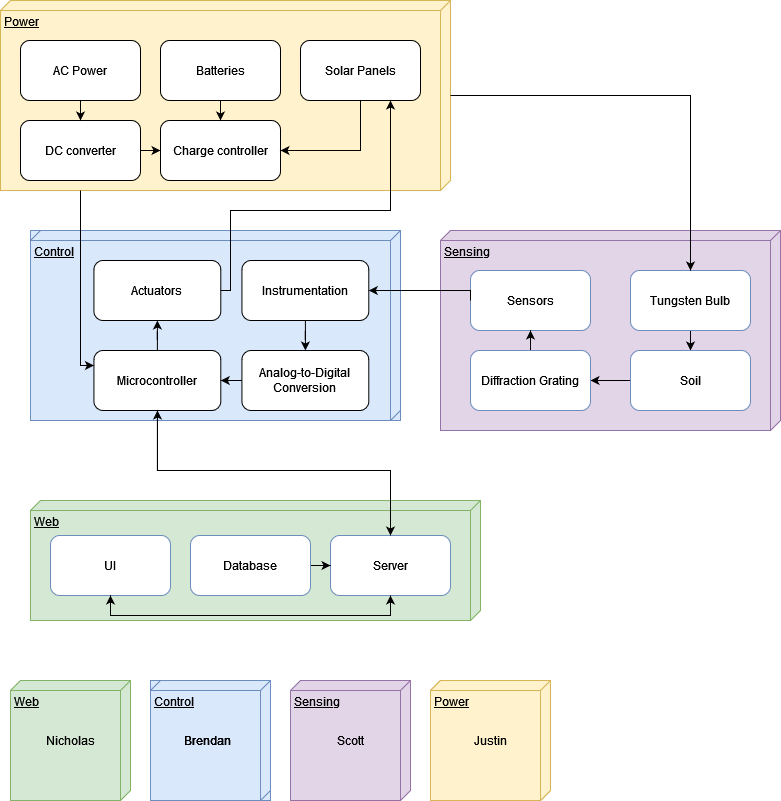
\includegraphics[width=\textwidth]{images/Overall Block Diagram.png}
    \label{fig:overall-block}
\end{figure}
\paragraph{Control}
The control subsystem is the brains of the entire operation. This subsystem has to accomplish four distinct tasks:
\begin{enumerate}
    \item Actuate mechanical components (linear rail, solenoid valve)
    \item Convert analog sensor data to digital data
    \item Send plant bed telemetry to web subsystem
    \item Receive commands from web subsystem and modify system accordingly
\end{enumerate}
In order to accomplish the first task, the chosen microcontroller (MCU) must be capable of driving the currents for these components and also support pulse-width modulation (PWM) for interacting with the motor controller. The second task requires that the MCU have an analog-to-digital converter. The third and fourth tasks necessitate WiFi connectivity as well as firmware support for either HTTP requests or WebSockets. These requirements for the control subsystem weigh heavily in the discussion of which MCU to choose found in Section \ref{sec:ps-control}.
\paragraph{Power}
The power system's function is self-explanatory, supply power to the entire system. This will be accomplished in two ways. First, using a DC barrel-plug to the wall, the system could be powered this way. The second way, is via the solar panels, batteries, and charge controller. Both manners of supplying power to the system must be regulated. Discussed in Section \ref{sec:ps-power} are the different ways that the charge controller can efficiently switch between battery power and the panels to increase battery health and charge level.
\paragraph{Sensing}
The sensing subsystem is where the majority of the novelty of this project lies. A lot of problems with electronic sensing is decay in the wet environs of plant beds. To improve upon this problem and hopefully offer a more sustainable and expandable approach, the team is going to try to accomplish sensing optically via infrared spectroscopy. Through the use of spectroscopy the team will be able to collect a wider range of data than just soil moisture content which includes soil OH group content, temperatue, and acidity.
\paragraph{Web}
The web component of this project accomplishes three things; data analysis, reporting, and user specified control of components. The data analysis is occurring on the web because of the greater availability of compute power and greater ease of programmability. For reporting, the web will use databases to store data ad infinitum and serve this data in the form of graphs or ``live'' metrics. The web component also will be able to take a user's input to send commands back to the control system to actuate different parts such as the solenoids or to ask for a more recent data reading.
\subsubsection{Engineering Specifications}
The team compiled a set of specifications for each of the subsystems that would need to be implemented to accomplish the requirements from above. \autoref{table:eng-specs} shows breaks down these specifications by the corresponding subystem.
\begin{table}[H]
    \caption{Engineering Specifications}
    \centering
    \begin{tabular}{c|c|c}
        \hline
        \textbf{Subsystem} & \textbf{Metric} & \textbf{Specification} \\\cline{2-3}
        \hline
        \multirow{8}{*}{\textbf{Control}} & Input voltage & 2.8-5.5 V \\ \cline{2-3}
                                        & Power consumption & $\leq$1.50W nominal power draw \\ \cline{2-3}
                                        & Shutdown power draw   & $\leq$100 uW \\ \cline{2-3}
                                        & Processor speed       & $\geq$20 MHz \\ \cline{2-3}
                                        & ADC resolution        & $\geq$8-bit \\ \cline{2-3}
                                        & ADC sampling rate     & $\geq$1 ksps \\ \cline{2-3}
                                        & Transmit power        & $\geq$10 dBm \\ \cline{2-3}
                                        & Receive sensitivity   & $\geq$-50 dBm \\ \cline{2-3}
        \hline
        \multirow{5}{*}{\textbf{Power}} & Power & 20-30W \\\cline{2-3}
                                        & Battery Capacity & 8Ah/95Wh \\\cline{2-3}
                                        & Battery Nominal Voltage & 9.6-12.8V \\\cline{2-3}
                                        & Charging Time & \textless4 hours \\\cline{2-3}
                                        & Regulator Efficiency & \textgreater65\% \\\cline{2-3}
        \hline
        \multirow{3}{*}{\textbf{Sensing}} & Spectra & 400nm - 1700nm \\\cline{2-3}
                                        & Resolution & \textless10nm \\\cline{2-3}
                                        & Output voltage range & 0-1.8V \\\cline{2-3}
        \hline
        \multirow{2}{*}{\textbf{Web}} & Up-time & 95\textpm.1\% \\\cline{2-3}
                                    & Storage Capacity & \textgreater16 GB \\\cline{2-3}
        \hline
        \multirow{2}{*}{\textbf{Miscellaneous}} & Dimensions & 1 m\textsuperscript{3} \\\cline{2-3}
                                                & Weight\tablefootnote{The weight of the system includes a full soil load} & \textless 50lb \\
        \hline
    \end{tabular}
    \label{table:eng-specs}
\end{table}
\paragraph{Control}
The specifications in the control portion of the table are focused on integrating the various subsystems in this product. Input voltage must be flexible to take either 3.3 V or 5 V as an input, plus or minus 0.5 V to account for possible fluctuations in power. The controls subsystem must not consume a large amount of power under nominal conditions to increase battery life and decrease battery size and capacity (and as a result, cost). Shutdown power draw must also be minimal, especially when the battery is completely drained. If the controls subsystem continues to draw from the battery past its rated capacity, the product may become a danger to the user. The processor must be fast enough to handle multiple operations concurrently and in a timely manner, while still being able to drive the network stack and wireless elements. The analog-to-digital converter must have a large enough resolution to accurately take measurements from the sensing subsystem, and must be able to sample sufficiently fast enough to take those measurements in fast enough succession to where they will be useful for our product. Transmit power must be ample enough to operate on a normal consumer WiFi network, and the receiver must be adequately sensitive enough to operate outside, away from the user's wireless access point.

\paragraph{Power}
The power specifications were made throughout the design process. For example, the power output was an unknown until all the subsystems had a firm idea of their power requirements. The maximum instantaneous power draw of the entire system is in the 20-30W range, hence where that specification is drawn from. The battery capacity and charging time are derived from the duration the team decided the system should last on battery power and the input power from the solar panels.

\paragraph{Sensing}
The spectra was chosen 

\paragraph{Web}
The web engineering specifications were hard to put into words. In general, the team wanted a reliable service quantified by the up-time of the web service. The service also needs to be able to store data in perpetuity for at least a single plantbed. Due to the efficiency of data storage and compression as well as the frequency of scans, the team felt that 16GB was effective enough to showcase the full system for now.

\paragraph{Miscellaneous}
The current miscellaneous specifications regard the physical qualities of the system. The dimensions of a meter cubed are necessary for the depth needed for various plants as well as solar panels. The weight is heavily correlated to weight of batteries, control and sensing components, as well as the soil and water hosing system. 
\subsubsection{Marketing Requirements}
When thinking about the target market for a project like this, the team put together a list of requirements important to the consumers. The most important feature for the consumer would be how easy the product is to use and navigate. This feature ranks the highest and would be the main determining factor on whether a consumer purchases this product over a competitor. Two other highly important features to a consumer would be the accuracy of the product and the cost. The accuracy is important because it directly correlates to the success of the customer's garden. If the product is not accurate in watering the plants, the customer will be unsatisfied and the plants will not survive. Cost because every consumer has to consider their budget - how much they are willing to spend for the features they deem most important. Other customer requirements the team brought up include the durability, configurability, environmental friendliness, portability and update frequency; listed from more important to less for consumer preferences. Each of these requirements have a direct correlation to at least one of the engineering requirements set for the product. \\

The engineering requirements set by the team are: weight of the product, dimensions of the product, battery life, how much power it consumes, up-time of the website, and quality of sensor resolution. \\

Many of the engineering requirements are directly correlated with each other. As weight improves, or lessens, so will product dimensions and vice versa. As dimensions decrease for the product, the amount of power needed decreases which means power consumption lessens which is also a positive correlation for the requirements. The only negative correlation in the engineering requirements the team found was that as sensor resolution increases, the life of the battery decreases as the lighting for the sensor must remain on longer. \\
 

\begin{figure}[H]
    \centering
    \caption{House of Quality}
    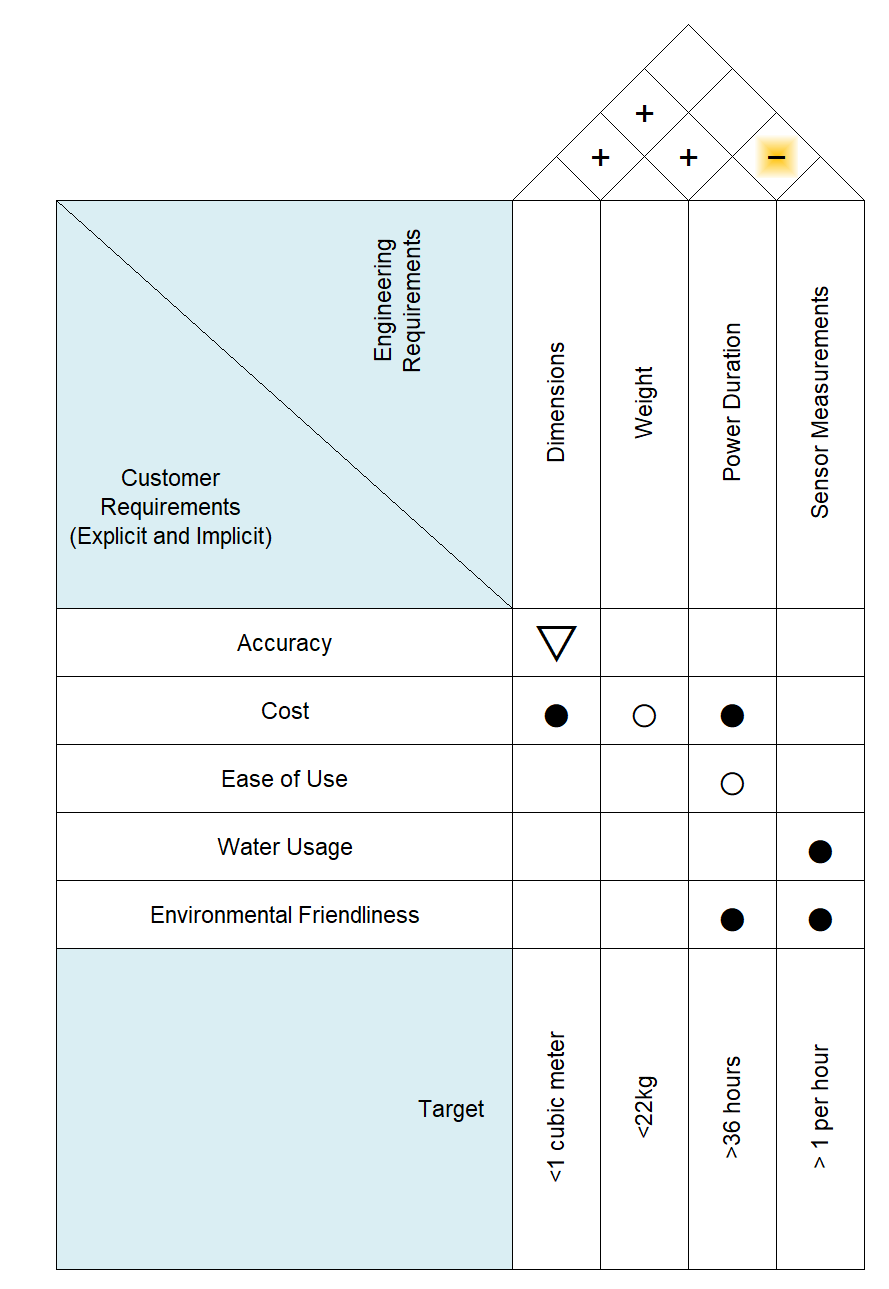
\includegraphics[width=\textwidth]{images/HouseOfQuality.PNG}
\end{figure}

When considering the customer requirement of ease of use, the team considered the impact of all the engineering requirements. Weight, battery life, and up-time all have a positive impact on customer experience. The lighter the product is, the easier it is for the customer to use because they can move it and adjust things within the product easier. The longer the batter life, the less time the consumer needs to worry when there are days with lower sunlight because the batteries can withstand a longer duration without being recharged. When the product has more up-time, the less time the consumer has to spend waiting on product updates. One of the engineering requirements that has a moderate impact on the customer experience is the sensor resolution. Although it can make a large impact on the overall product performance, its direct correlation to ease of use is not as strong as other requirements. The second most important marketing requirement listed by the team was accuracy. The only engineering requirement that had any correlation, had a strong correlation which is sensor resolution. This requirement is important to this marketing requirement because it could be a tipping point on whether a consumer purchases this product versus another. If the sensor resolution is not high enough to detect watering needs for the plant, the product will not be successful. This is why it is such an important requirement to focus on for both marketing and development of the product.\\

Something every team and every consumer is going to consider when designing or purchasing a product is the cost. The team rated this marketing requirement as an 8/10 for this product. It was not the highest priority because for a product like this, consumers will pay more to have a more accurate and easy-to-use product. The team also considered that customers using this product will do more research about the technical features because they are most likely growing fruits or vegetables that they will consume. Unfortunately, most things that increase the quality and appeal of the product, have a negative relationship that is strong in correlation. When the team looks at lighter materials, those materials increase the price. When adding a longer battery life and lowering power consumption, price will increase proportionally to how much those requirements change. To increase the resolution of the sensor, the team and consumers will have to pay more for the increase in quality and performace. The only requirement that  correlates to cost that was not strong, but still has an impact is the up-time. The more up-time of the product services, the more cost that is involved, but it is a smaller margin compared to the other requirements that directly impact the cost of the product. \\

Durability is most affected by the engineering requirements of weight and dimension. If the product materials are different, the durability will change and if the dimensions change shape or length, the construction will change affecting product strength. Weight will have a stronger impact on durability because it is something cosumers will consider more heavily and the materials will impact more. This is why weight has a strong correlation and dimensions are moderately correlated. Another marketing requirement that is similarly affected by weight and dimension is the portability of the product. The battery life also affects the portability. As battery life increases, so does the size and configuration of the battery which affects how easy it is to move. Weight has the largest affect on portability, followed by dimensions and then battery life. The configurability of the project is strongly affected by both dimension and power consumption. Battery life has a smaller affect on this, but still changes the set-up of the product. \\

Although environmental friendliness rates lower on the consideration for a consumer, it is affected by more engineering requirements. Battery life has a small impact on how environmentally friendly this product is because of the waste that will exist once the battery is retired. The factor considered most impactful is the power consumption. The greater the power consumption, the less friendly the product will be to the environment. If the team is able to focus on lowering the power consumption, marketing will be easiest for environmental friendliness. Up-time and sensor resolution have a moderate affect on this requirement and should have some connsideration in design of the product, but will be considered with more correlation to other requirements than environmental impact. \\

The last requirement comparison done by the team is update frequency. This marketing requirement is strongly correlated to up-time and moderately correlated to sensor resolution. Both of these engineering requirements affect the time spent on updating the software for the product. \\

\paragraph{Competition}
This product already has a competitive edge in the current market because it is unique. It will be the first all-inclusive garden bed that can be used outside. When looking at products that offer something similar, the team found two main options that a consumer may consider next to this product. The first competitor being considered is the Aero Garden. This product is a small indoor herb garden that provides UV light to help the plants thrive. A consumer wanting to start only an herb garden indoors may consider this product because it is more affordable, but would choose our product for its ease-of-use. The full garden bed design is more durable and waters the plants for the consumer. This is a big factor for a consumer to consider because many gardeners over or under water their plants. So although the Aero Garden may be more competitive indoors, the target market for our product will be won over with the requirements our team has focused on. The second competitor we considered is the FarmBot. This product is an automatic watering system that can be installed on an outside garden bed. When consumers glance at both of the products, they will automatically lean towards ours because of the value and price point. The FarmBot may have more accuracy, but not significant enough to justify the price difference. Additionally, this product is harder to assemble and larger which won't accomodate the average home-gardener. FarmBot is for a consumer that has more time, space, and money, but not for the majority of consumers.    % Section 2.3 - needs work, expanding requirements, better house of quality
\section{Research}                              % Section 3
Our research covers three core components: previous works, related technology, and part selection. 
\subsection{Previous and Related Works}
These are projects that accomplished similar objectives to what we hope to accomplish or highlight a technology we plan to work with.
\subsubsection{DIY near-IR spectrometer}
Yuan Cao is a Ph.D. student at MIT with a blog where he posts his unofficial projects. He published a project titled “A \textdollar500 DIY near-IR spectrometer that would sell for \textdollar10,000.” In it, he describes his idea, designs and results for a low cost infrared spectrometer. His design features surprisingly high performance for its price. The system uses an InGaAs photodiode, a reflective diffraction grating, a fiber collimator, some cheap optics, and a microcontroller to create a spectrograph of any light source. It boasts very high signal to noise ratios, 5-6nm spectral resolution, and a price point under \textdollar500. There are definitely some design features worth imitating, specifically the diffraction grating “scanner” that is rotated to pass wavelengths across the surface of the photodiode, as well as the filter circuitry that cleans up the electrical signal. 
\begin{figure}[H]
    \caption{NIR Photodiode Spectral Sensitivity}
    \centering
    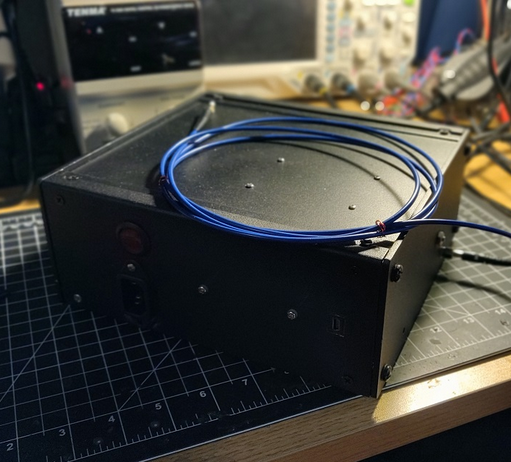
\includegraphics[width=\textwidth]{images/3.1.1Pic.png}
\end{figure}
That said, there are some reasons why this project differs in application from the Auto Garden Bed Near Infrared Spectrometer. First, the detector has a spectral range from 800 – 1600nm. This is the Near Infrared Regime, but it is not very far into the NIR, which in some contexts refers to wavelengths as far out as 2500nm. If Soil Spectroscopy requires this depth, or frequencies in the visible spectrum, the design will have to be modified. Second, this system was built for lab use, specifically to characterize light sources. The reported data was very promising, but in every case the spectrometer targeted an object that was emitting strong optical power in every direction. Soil does not fluoresce, so the Auto Garden Bed will require additional components to probe the soil with an electromagnetic wave. In the end, what’s most important is that this project demonstrates that low cost spectroscopy can be achieved.


\subsubsection{Chlorophyll Flourescence Spectrometer}



In 2021 UCF’s ECE Senior Design Group 1 designed a Chlorophyll Fluorescence Spectrometer. The purpose of this project was to design a system that would detect chlorophyll in plants through stimulation by UV rays. It featured a diffraction grating and a monochromatic CMOS sensor. It is interesting to note that unlike the previously explored project, spatial separation of light frequencies is achieved with a monochromatic camera. This means that each intensity can be mapped to the position on the cmos sensor, and the system can “stare” rather than “scan.” Eliminating moving parts is a major benefit in projects requiring sensitive optical alignment, making this a feature worth seriously considering.

\begin{figure}[H]
    \caption{NIR Photodiode Spectral Sensitivity}
    \centering
    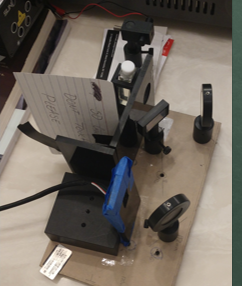
\includegraphics[width=.6\textwidth]{images/3.1.2Pic.png}
\end{figure}

This project produces a design with similar goals to the Auto Garden Bed, because it features a light source, a target object, focusing optics, wavelength selection, and generating and interpreting a spectrograph. However, the optical regime of UV rays may be limited to fluorescence spectroscopy and unfit for proximity soil sensing. The research will have to determine what sensors are viable and whether this imposes further constraints on the system.

\subsubsection{Smart Garden Controller}
The Smart Garden Controller was a UCF senior design project with very similar motivations to the Auto Garden Bed. The goal was to create a system that reduced user labor by automating the irrigation schedule of garden areas and reducing waste by sensing moisture levels. The system was also designed to anticipate the informational needs of the gardener and come prepared with a set of popular vegetables and plants, corresponding to variables the team had already investigated to maximize flourishing. It used sensors to detect the health of the plant environment, a microcontroller to facilitate irrigation, and a web API to interface to the user for control of the system. The group also set goals to offer ease of setup, competitive price, and Smart Device integration by integrating with a device like Amazon’s “Alexa.” The last similar design features are wall plug power consumption, lithium ion battery backup power, and http secure information protocol over wifi.
\begin{figure}[H]
    \caption{NIR Photodiode Spectral Sensitivity}
    \centering
    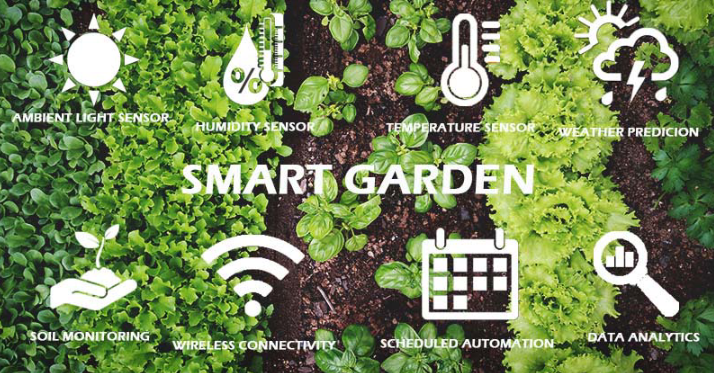
\includegraphics[width=\textwidth]{images/3.1.3Pic.png}
\end{figure}
This project features much of the same core functionality as the Auto Garden bed, however, closer review of the scope and feature set reveal that the designs are incompatible. The Smart Garden Controller was designed to facilitate more precise control of an entire garden, allowing the user to isolate different areas for growing different plants. The area of interest was 100 squared feet, and the system was intended to relieve the gardener of the complication of watering each section for different amounts of time. This meant a wide reaching irrigation network as well as a network of sensors throughout the yard. The scope of the Auto Garden Bed allows for single source irrigation and sensing, which allows for greater flexibility of mechanical design, including power generation and environmental controls.

\subsubsection{Automated Rotating Solar Plant Rack with Self-care Capabilities}

This is another home garden system with a different target solution. The goal is to facilitate the growth of indoor plants and ensure maximum plant health by rotating the plant base so that the forces driving it to grow sideways cancel out in every direction. Like previous projects, the system is integrated with wireless communication and a schedule selector for different plant types. Unlike previous projects, one of the means of achieving plant health is by protecting sensitive plants from excessive exposure to sunlight, which is a feature that the Auto Garden Bed seeks to implement. 

\begin{figure}[H]
    \caption{NIR Photodiode Spectral Sensitivity}
    \centering
    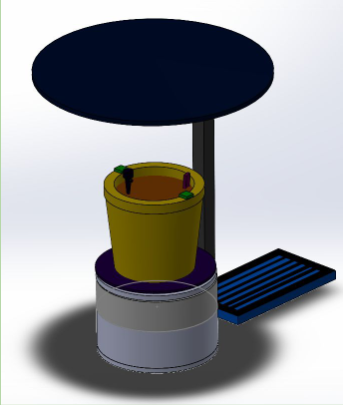
\includegraphics[width=.6\textwidth]{images/3.1.4Pic.png}
\end{figure}

Another point of interest in the Automated Rotating Solar Plant Rack is its rotating foundation. Maximizing sun exposure is a goal of this project, and although the application is energy collection, there may be parallel design opportunities with the Solar Plant Rack.


\subsubsection{Stem 'n' Leaf}
Stem 'n' Leaf\footnote{https://www.ece.ucf.edu/seniordesign/sp2021su2021/g07/} is a UCF Senior Design project. The focus of this project was to be a ``modular hydroponics system'' wherein each plant unit can be fed my a singular control unit. Thus, the ``stem'' is the control unit and the ``leaves'' are the plant units. Their design was focused on modularity and scalability. Hence their design is stackable and tileable design of the bed itself. The key features of this plant bed is that it self-regulates pH and integrates with a mobile application.
\begin{figure}[H]
    \caption{NIR Photodiode Spectral Sensitivity}
    \centering
    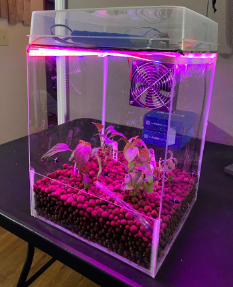
\includegraphics[width=.6\textwidth]{images/3.1.5Pic.png}
\end{figure}

The project uses a liquid pH-sensor to obtain the relevant data. Our team wants a similar result but will be trying to achieve this via optical means. Their team mentioned the durability of the sensor which is our team's chief concern seeing as acidic and basic solutions tend to be corrosive and promote oxidation of metals thus the optical approach should improve longevity of the project. 

\subsubsection{Green Steel Garden}
Green Steel Garden\footnote{https://www.ece.ucf.edu/seniordesign/su2021fa2021/g11} is another UCF Senior Project that our team is pulling some inspiration from. Another hydroponics system that measures soil nutrients and pH for controlling the parameters of the garden bed. The key feature of this project is the nutrients system and the pH sensor.

\begin{figure}[H]
    \caption{NIR Photodiode Spectral Sensitivity}
    \centering
    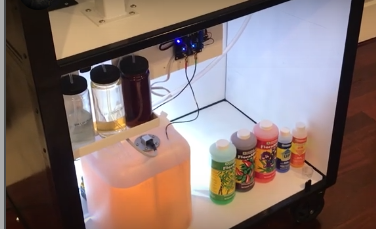
\includegraphics[width=\textwidth]{images/3.1.6Pic.png}
\end{figure}

This project utilizes a water reservoir and reservoirs of chemicals to balance the pH of the water entering the garden bed. They use peristaltic pumps to accomplish the mixture and a combination of pH and electrical conductivity sensors to get data from the water. The current design consensus for our team is that we will be hooked up to hose which is limited by a solenoid valve, but being able to ``treat'' the water that is entering the system may be a design decision that has to be considered.

\subsubsection{Summary}

The previous works discussed here highlight the key components of our garden bed: sensing in conjunction with optics. Something of note in these deliberations is the use of hydroponics in all of these projects; something that is rendered unnecessary and seemingly inefficient in an outdoor garden bed.

The previous works related to optics focus on wavelengths outside of our team's consideration (Infrared), instead focusing on UV and visible light through near-Infrared. Their research highlighted potential flaws in some assumptions we had made. Firstly, that it is possible to reduce the moving components of our optical sensing, obtaining a wider field. Secondly, that using IR spectroscopy is practical for getting data from soil as it is used in commercial projects today and shows tremendous value in commercial sectors.

Most of the other garden bed projects focus on hydroponics but something of interesting note is the rotating solar rack project. The control scheme regarding the degrees of rotational freedom and the means of achieving success will be paramount in implementing our own moving solar array. Of interesting note is that all the other garden bed projects focused primarily on hydroponics as it gives greater measures of control to the soil nutrients which had not been a consideration of our team before looking into the previous works. Instituting a chemical pump into our design may be necessary to achieve our goal of being ``set it and forget it'' while still providing updates for when to refill the chemical tanks of integration with the water.

All of the garden projects tried to integrate some means of a mobile app or web user interface. They all mentioned that they needed to have started this component earlier. Each of the mobile application projects were not able to achieve this by their final meeting which is of special concern. Also of note is their choice of stack; many of the projects chose a NoSQL stack which seems counterintuitive given the highly relational nature of the data that is being collected. Our team can learn from this by starting this integration as early as possible and choosing to implement the smallest possible feature set that accomplishes the goals.
              % Section 3.1
\subsection{Related Technologies}
TBD, DESCRIPTION NEEDED HERE.

\subsubsection{Ocean insight: Ocean ST NIR Microspectrometer}

Ocean Insight is a local manufacturer of high-end, low size, weight, and power spectrometers. The ST NIR Microspectrometer is about 40 cubic centimeters in volume with a scan speed of 10ms, a signal to noise ratio of 190:1, and a spectral resolution of 2.2nm. Its spectral range is from 645nm to 1085nm, and it was specifically designed to be integrated into larger systems for customers who were interested in a flexible, low-cost design. Added to that, the system is rugged, and offers a variable slit input size, increasing its flexibility even further. While the designs are proprietary, this system serves as a benchmark for what can be achieved by the industry, and no doubt there are major design changes that can be made to achieve a similar result for the application intended for the Auto Garden Bed. That being said, the selling price for one is \textdollar1,750.

\begin{figure}[H]
    \caption{Ocean ST NIR Microspectrometer}
    \centering
    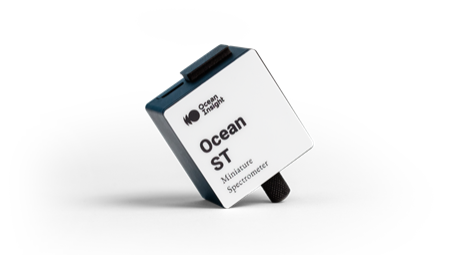
\includegraphics[width=0.5\textwidth]{images/3-2-1Pic.png}
\end{figure}

\subsubsection{AgroCares Nutrient Soil Scanner}

AgroCares offers a Near Infrared Spectrometer specifically designed for Proximity Soil Sensing. Its spectral range is from 1300 to 2500nm and it uses Micro Electrical Mechanical Systems or MEMS to capture EM Waves reflecting off the soil. The real value of the product is in its wireless communications system. The device uses Bluetooth 4.0 to send data to a cloud data center. There, spectrographs of large data sets of soil with known nutrient contents are compared with the reading, cutting out the need for on-sight calibration. The system is handheld and uses eight tungsten halogen bulbs to blast the soil with energy. This light is collected in an extremely small area, sampling 65 squared millimeters. It would be worth researching to see if the Tungsten bulbs were linked to the 1300 to 2500nm spectral range or if another probe and sensor would suffice.

\begin{figure}[H]
    \caption{AgroCares Nutrient Soil Scanner}
    \centering
    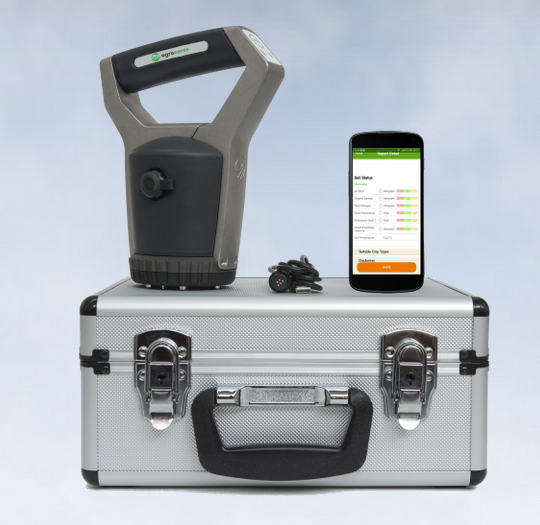
\includegraphics[width=0.5\textwidth]{images/3-2-2Pic.png}
\end{figure}

\subsubsection{DIY Webcam Diffraction Grating Spectrometer}\label{sec:DIYTransmissionGratingSpectrometer}

Physics Open Lab is a blog posting site for do-it-yourself physics laboratory projects. This project makes use of a megapixel webcam and a 1000 line/mm transmissive diffraction grating. The megapixel sensor allows for “staring” scanning, which is used in conjunction with spectrograph software for identifying the wavelength bands as they spread out from the zero order transmission. The project offers some interesting ideas, from the use of open source spectroscopy software to the use of two dimensional spectral analysis. Unfortunately, the use of a transmission grating presents a major problem for this application. Transmission gratings output most of their optical power straight ahead, and they are difficult to separate as higher order groups. While the project results where impressive, it did not generate a single spectrograph past the 1um range, which is necessary to detect the Moisture Content of the Soil.

\begin{figure}[H]
    \caption{Webcam Transmission Grating Spectrometer}
    \centering
    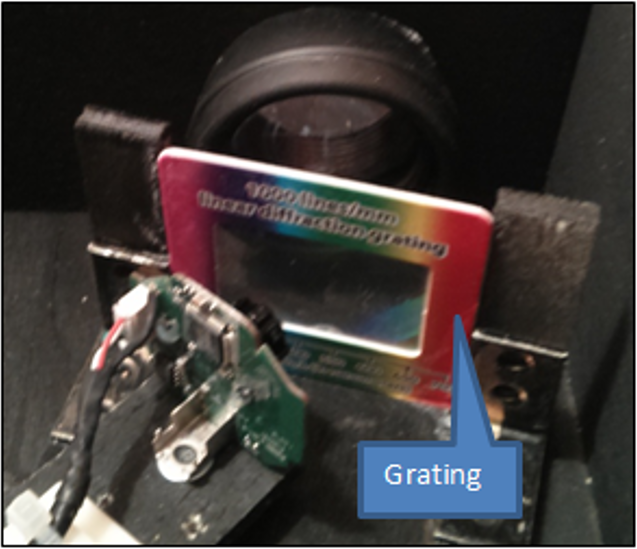
\includegraphics[width=0.5\textwidth]{images/DIYTransmissionGratingSpectrometer.png}
\end{figure}

\subsubsection{Web Technologies}\label{sec:web-tech}
\paragraph{Docker}
``Docker is a platform designed to help developers build, share, and run modern applications. We handle the tedious setup, so you can focus on the code.'' This quote comes directly from Docker's website on why developers should switch to Docker. This technology makes items more portable by making the executable platform agnostic through the use of a docker kernel and containers. The figure below should provide some clarity:

\begin{figure}[H]
    \caption{Docker architecture}
    \centering
    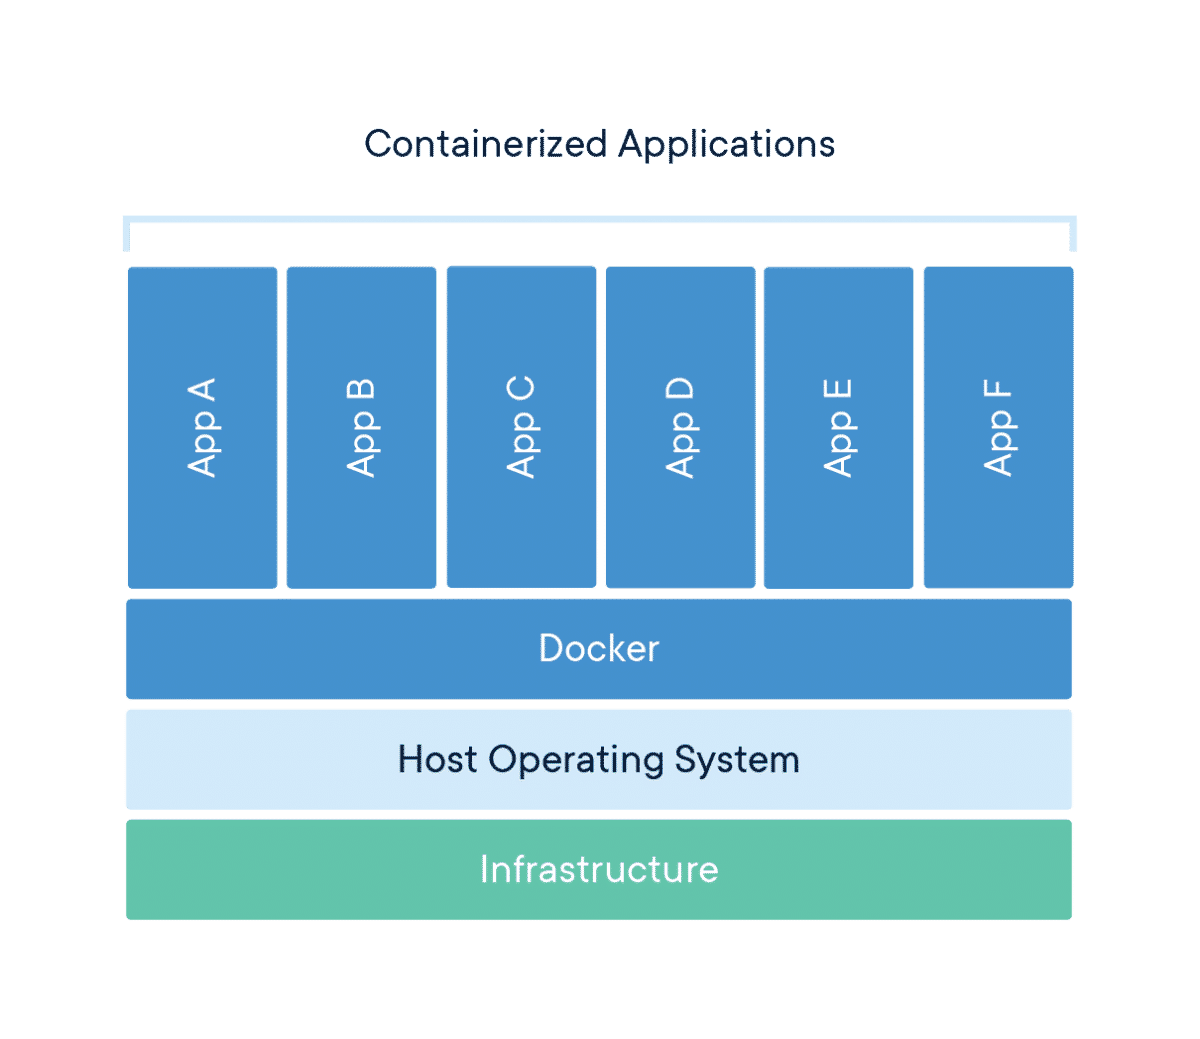
\includegraphics[width=\textwidth]{images/Docker-Architecture.png}
    \label{fig:docker_arch}
\end{figure}

A developer can program applications such as those demonstrated in figure \ref{fig:docker_arch}, package them into images and run them in containers. Docker works with the OS kernel to provide the same environment to the application each and everytime.

One of the largest advantages to using and implementing Docker that the team sees is that one team member can program and package the image and it should ``just run'' on any other team member's machine. This fact will prove very useful in integration testing especially for the socket server detailed in Section \ref{sec:web_subsystem}.

\paragraph{User Interface}
Because these are web technologies we will be using Javascript frontend frameworks/libraries for creating the frontend. Based upon cursory research, the most feature-rich and most widely used are React and VueJS.
\subparagraph{React}
React is a component-based library for building user interfaces.  Many libraries have extended the functionality by adding components to React for use by other developers. A React component is a stateful element in the Document Object Model (DOM). Essentially, based on the state information, a component is rendered in raw HTML to the browser. One such example of a component library is MaterialUI (MUI). MUI is a popular library for adding components like hamburger menus, tables, graphs, etc. Choosing React decreases the time spent developing due to the ease of tossing boilerplate components at the problem. The biggest issue is that all rendering is done in the browser which means that loading an uncached page may take a long time. Frameworks built ontop of React such as NextJS help speed up this process by moving some of the processing to the server.
\subparagraph{VueJS}
VueJS is a framework for building user interfaces. The difference between a library and a framework is that a framework provides a control flow while libraries are just used. VueJS is not too unlike raw HTML and JavaScript wherein \verb|<script>| tags are used to create dynamic pages in response to user actions. The key difference between Vue and the above is that Vue provides the access to component-based programming. Similar to React, Vue works on the basic of components but it uses the default HTML DOM and adds functionality to pre-existing components. This comes with the limitation that components are not nearly as interleaved with data from a web server. Vue is performant and designed for single-page applications, which may not server this project well in the long-run.
\paragraph{Web and Socket Server}
This section will host information related to technologies for building out a web and socket server for connecting the user interface to the backend. .NET, Java and JavaScript all have reasonable solutions to these but based on the JavaScript user interface, this discussion will be kept to Java and JavaScript solutions and technologies.
\subparagraph{Java Spring Boot}
Java Spring Boot is a full featured library that has different webservers embedded such as Apache Tomcat. Web servers are the means for which an application can be accessed from the outside world. Java Spring Boot makes this process incredibly easy. Part of this project will be communicating via TCP packets as well as through HTTP requests. Java at first glance seems like the easier way of accomplishing both tasks through the \verb|java.net| libraries and through the use of Spring Boot \verb|@Controller|.

The \verb|java.net| libraries are essentially a port of the network protocols that were made in the C language for creating communications via packets. By deploying using Java Spring Boot, it is possible to create two services packaged into one, the socket server and the web server. Java's memory management and VM environment leave a lot to be desired. The current state of the language and its artifact leave a lot to be desired as well. Because of the nature of running as a server and potentially servicing multiple plant beds, Java's lack of callbacks and lacking multi-threading support means it is downgraded given its overhead.

The \verb|@Controller| is such a great feature in Spring Boot. Java is strictly typed, leading to a lot really helpful features in executing backend requests. Also, because of the overhead, Java ORMs tend to be more fully featured and have support for a variety of other tools that increase velocity when programming. One such tool is Liquibase. Liquibase is a database changelog tool for creating and implementing database migrations based on a code.

\subparagraph{ExpressJS}
Express is a lightweight backend framework for implementing routes and middleware in JavaScript. The biggest disadvantage of using Express is the lack of low-level capabilities. Express was designed to be multiple layers of abstraction away from the kernel which may prove to be tumultuous when trying to create a socket server that communicates with the MCU.
\paragraph{Databases}
A database is essential for tracking data and persisting it for use later. There are two main types of database, SQL and NoSQL. With these two types of database comes a variety of implementations and on top of that a variety of tools to work with them. Let's compare SQL vs NoSQL first.

\begin{figure}[H]
    \caption{Difference between SQL and NoSQL}
    \centering
    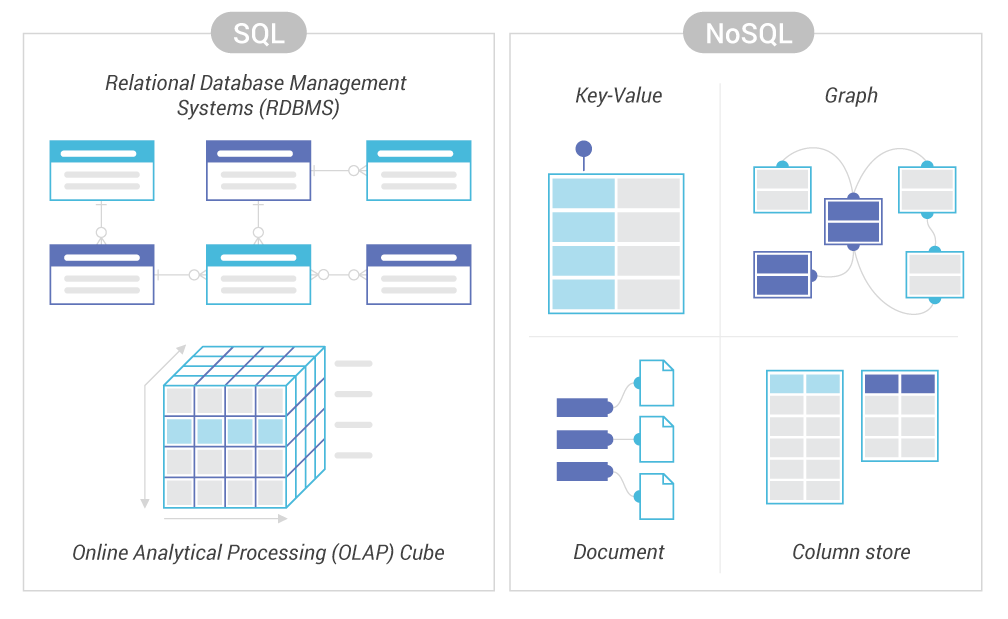
\includegraphics[width=\textwidth]{images/SQL-vs-NoSQL.png}
    \label{fig:sql_vs_nosql}
\end{figure}

\subparagraph{SQL vs NoSQL}
In Figure \ref{fig:sql_vs_nosql} you can see the abstracted way to think about these two different systems. SQL records are exactly that, a record at a point in time. If one entity encapsulates another then another table holds that information. In NoSQL, the information is abstracted to a document with key-value pairs to get specific data. These documents can make references to other documents but for time-ordering this is highly ineffective. SQL records are highly effective for logs and indexing a large amount of data based on a higher level entity such as user that has many garden beds; garden beds that have a lot of data, etc.

\subparagraph{MySQL vs PostgreSQL}
The two SQL databases widely used in industry are MySQL and PostgreSQL. MySQL is touted as ``a simple relational database [... that is] very efficient and user-friendly'' while PostgreSQL is widely used in data analytic and scientific applications because of the extensibility, scalability and object models. Immediately this seems like the better option but PostgreSQL may be harder to stand up immediately. Special consideration should be given to AWS solutions as well. 

\subparagraph{MongoDB vs DynamoDB}
MongoDB is ``a general-purpose, document-based'' database. DynamoDB is AWS' proprietary solution to NoSQL databases. DynamoDB is more difficult to work with as it is the newer service, it could also potentially be more expensive over time, however, DynamoDB has improvements over MongoDB for indexing and building out reference documents. 

\subsubsection{Proportional-integral-derivative Control}
Proportional-integral-derivative control (PID control) is a common control algorithm (espectially in industrial control systems) to allow a control loop to have reliable performance in a variety of conditions. Simply put, this algorithm allows a controller to receive an input and calculate a proportional output, accounting for error and rapid changes in the process. This algorithm may be useful to our application because it will allow the product to better control its facilities without user input.

The control function is defined in \autoref{eq:pid_controller}, where $u(t)$ is the control variable (e.g. the garden bed's water control solenoid), $K_p$, $K_i$, and $K_d$ are gain factors, and $e(t)$ (the error) is the different between a desired setpoint and measured process variable (e.g. the difference between the desired and current ounces of water dispensed).
\begin{equation}
    \label{eq:pid_controller}
    u(t) = K_pe(t) + K_i\int_{0}^{t}e(\tau) \, d\tau + K_d\frac{de(t)}{dt}
\end{equation}

\paragraph{Proportional Term} The proportional term of \autoref{eq:pid_controller} is $K_pe(t)$, hence referred to as the P-term. The P-term is proportional to the current error, and the gain $K_p$ determines the magnitude of the P-term. If the gain is too large, then the process variable will oscillate.

\paragraph{Integral Term} The integral term of \autoref{eq:pid_controller} is $K_i\int_{0}^{t}e(\tau) \, d\tau$, hence referred to as the I-term. This term accounts for previous values of $e(t)$ by taking the integral of the error, and the gain $K_i$ determines the magnitude of the I-term. The I-term aims to account for residual error in the control loop.

\paragraph{Derivative Term} The integral term of \autoref{eq:pid_controller} is $K_d\frac{de(t)}{dt}$, hence referred to as the D-term. The D-term aims to control future values of $e(t)$ by taking the derivative of the error, and the gain $K_d$ determines the magnitude of the D-term. This term acts to damp rapid changes in the control loop. Higher values of gain may make the control loop more sensitive to noise and lead to instability.                 % Section 3.2
\subsection{Part Selection}
\subsubsection{Controller Subsystem}
\begin{flushleft}
	At minimum, any chosen microcontrollers (MCUs) shall support natively, or by addition of a
	module, these features and traits:
	\begin{itemize}
		\item Analog-to-digital converter (ADC)
		\item cURL compatibility
		\item IEEE 802.11
		\item In stock and available to order
		\item JTAG module or equivalent
		\item Module communication bus (UART, I2C, SPI)
		\item Onboard CPU sufficient for our purposes
		\item Onboard memory sufficient for our purposes
		\item Onboard nonvolatile memory
		\item Pins dedicated to analog input
		\item Pins dedicated to digital I/O
	\end{itemize}
	These features would be "nice to have" on any MCU selected, but are not required:
	\begin{itemize}
		\item Digital-to-analog converter (DAC)
		\item microSD card slot
		\item Onboard battery
		\item Pins dedicated to pulse-width modulation (PWM)
		\item Timer(s) and an RTC
		\item USB compatibility
		\item Additional wireless communication protocols (e.g. BT or BLE, Zigbee)
	\end{itemize}
\end{flushleft}
\begin{flushleft}
	The selections, listed in \autoref{table:mcubreakdown1} and not in any particular order, match
	the above criteria and are being considered for selection.
	\begin{table}
		\centering
		\begin{tabularx}{\textwidth}
			{
				| >{\raggedright\arraybackslash}X
				| >{\raggedright\arraybackslash}X
				| >{\raggedright\arraybackslash}X
				| >{\raggedright\arraybackslash}X
				| >{\raggedright\arraybackslash}X
				| >{\raggedright\arraybackslash}X
				|
			}
			\caption{MCU option breakdown}
			\label{table:mcubreakdown1} \\
			\hline
			\textbf{Model} & \textbf{\href{https://www.ti.com/tool/LAUNCHXL-CC26X2R1}{LAUNCH\-XL-CC26X2\-R1}} & \textbf{\href{https://www.ti.com/tool/LAUNCHCC3220MODASF}{LAUNCH\-CC3220\-MODASF}} & \textbf{\href{https://www.raspberrypi.com/products/raspberry-pi-pico/}{Pico W}} & \textbf{\href{https://store-usa.arduino.cc/products/arduino-nano-33-ble?selectedStore=u}{Nano 33 BLE}} & \textbf{\href{https://www.st.com/en/evaluation-tools/b-l4s5i-iot01a.html}{B-L4S5I-IOT01A}} \\
			\hline
			\textbf{Manu\-facturer} & Texas Instruments & Texas Instruments & Raspberry Pi & Arduino & STMicro\-electronics \\
			\hline
			\textbf{Micro\-controller} & CC2652R & CC3220\-MODASF & RP2040 & nRF52840 & STM32\-L4S5VIT6 \\
			\hline
			\textbf{Processor} & 1x ARM Cortex-M4F & 1x ARM Cortex-M4 & 2x ARM Cortex-M0+ & 1x ARM Cortex-M4 & 1x ARM Cortex-M4 \\
			\hline
			\textbf{Maximum Speed (MHz)} & 48 & 80 & 133 & 64 & 120 \\
			\hline
			\textbf{Memory (KB)} & 256 ROM, 352 flash, 100 SRAM & 1024 flash, 256 RAM & 16 ROM, 264 SRAM & 1024 flash, 256 SRAM & 2048 flash, 640 RAM \\
			\hline
			\textbf{Wireless capability} & BLE5.2, Zigbee, Thread & 802.11b/g/n & 802.11n & BLE5.3, Zigbee, Thread, Matter & BT4.1, 802.11b/g/n, NFC \\
			\hline
			\textbf{Serial capability} & UART, I2C, I2S, SPI & UART, I2C, SPI & UART, I2C, SPI, USB1.1 & UART, I2C, I2S, SPI, USB2.0 & UART, I2C, SPI, USB2.0 \\
			\hline
			\textbf{Price (\$)} & 40, maybe free & 60, maybe free & 6 & 28 & 53 \\
			\hline
			\textbf{ADC} & 8-channel, 12-bit & 4-channel, 12-bit & 4-channel, 12-bit & 8-channel, 12-bit & 16-channel, 12-bit \\
			\hline
			\textbf{Clock capability} & Timer, RTC & Timer, RTC, WDT & Timer, RTC, WDT & Timer, RTC, WDT & Timer, RTC, WDT \\
			\hline
			\textbf{GPIO (pins)} & 31 & 29 & 30 & 13 & 16 \\
			\hline
			\textbf{PWM (channels)} & Supported & Supported & 16 & 4 & 6 \\
			\hline
			% \textbf{AES (bits)} & 128, 256 & 256 & Not supported & 128 & 128 \\
			% \hline
			\textbf{Required voltage (V)} & 1.8 -- 3.8 & 2.3 -- 3.6 & 1.8 -- 3.3 & 4.5 -- 21 & 4.75 -- 5.25 \\
			\hline
		\end{tabularx}
	\end{table}
\end{flushleft}
\begin{flushleft}
	Use of single-board computers (SBCs) was considered, but will not not need to be used; cURL 
	used on an MCU in conjunction with \href{https://aws.amazon.com/ec2/}{Amazon EC2} services will
	allow us to offload computing to a cloud solution.
\end{flushleft}
\begin{flushleft}
	Use of an external Wifi module is discouraged due to the following:
	\begin{itemize}
		\item Added cost
		\item Added complexity
		\item Modules in common use by hobbyists often have poor or no proper documentation, to the
		extent of:
		\begin{itemize}
			\item Quick start guide
			\item User's guide
			\item Datasheets
			\item Theory of operation
			\item Application uses
			\item Troubleshooting guide
			\item Schematics and mechanicals
			\item Quality and reliability
			\item Errata
		\end{itemize}
	\end{itemize}
\end{flushleft}
\begin{flushleft}
	Therefore, all of the MCUs listed above support either the 802.11 or Bluetooth standards.
\end{flushleft}
\begin{flushleft}
	Ultimately, the \href{https://www.ti.com/tool/LAUNCHCC3220MODASF}{LAUNCHCC3220MODASF}
	was chosen as the microcontroller development board for this project. In the event that the
	aforementioned LaunchPad is not able to be obtained, the
	\href{https://www.ti.com/tool/CC3220SF-LAUNCHXL}{CC3220SF-LAUNCHXL} has equivalent capability
	for the project's needs.
\end{flushleft}
\begin{flushleft}
	These boards, henceforth referred to as the CC3220, are able to be requested from our
	university at no upfront cost to our team. This was the driving factor behind choosing 
	the CC3220 over other microcontroller development boards. It was also determined that
	the microcontroller \emph{must} be able to interface via the 802.11 (WiFi) standard, for reasons
	that are detailed in \autoref{sec:controller_subsystem}---therefore, the LAUNCHXL-CC26X2R1
	and Nano 33 BLE were disqualified from selection. The Pico W was considered due to its low cost,
	and the B-L4S5I-IOT01A considered because of its abundant peripherals, but both ultimately lost
	out to the Texas Instruments products.
\end{flushleft}
% End Controller Subsystem

\subsubsection{Power Subsystem}
\textbf{Power Supply}\par
The power system is a key factor to this model and trying to make this an independent system. This is key because this power system needs to be able to power all of the many different components, while also charging itself when not operating.\par
As part of the goal to make this an independent system, solar energy plays a great role in this and making this system run. Before anything as well, this part of the system must operate first before it can power other components. For this system to run, the key parts include: solar panels that convert light energy into electrical energy; solar charge controller to regulate output voltage from the solar panel into the battery; the battery to directly power the other components in the model.\par
In this model there are many different sensors, electrical, and mechanical components all of which require power. This requires a design of how the power system will flow and operate. It first begins with determining the total power needed for the whole system to run. This can be determined by finding the individual power ratings of each component and calculating them all together. After that is found, we can then choose what type of battery and the quantity needed for the model. When choosing what kind of battery and how many is needed, how long we want the system to run, optional secondary power source, and optional battery bank must be put into consideration as well. As follows, we begin to research solar panels from type, efficiency, power rating, etc. Then, a solar charge controller must be selected, a device that sits between the solar panel and the battery to regulate how much power is going into the battery. Once that is done, a voltage regulator must be determined, to regulate voltage from the battery to the smaller components that need to be powered. After all that is done, then we can find other components that will make the power system more reliable and efficient in any way.\par
\textbf{Power Requirement}\par
Sensors, electrical, and mechanical components all require power but all consume different amounts of power. As mentioned before, analyzing the total power requirement is important and crucial because this will help us determine the right parts that will be best for this system and for the components.  \par
With the total power determined, the Watts per hour needed for all of the components to run must also be found. The watts per hour is important too because this helps figure out how long each component will operate for. After that is found, we used the altE calculator to help pick out what kind of battery can be used, then solar panel and solar charge controller, respectively. The altE calculator is a great resource because with the proper measurements, it can help us choose what kind of battery we can use, by determining the capacity needed in watt-hours or amp-hours. This calculator can also help us choose how big of a solar panel we need and how big of a solar charge controller we need as well. \par
\textbf{Rechargeable Battery Selection}\par
Solely relying on solar energy isn’t always ideal. This is because the weather may not always guarantee sunlight, this will hinder its power retention. For this reason, solar panels are paired with a battery so that the power can be stored and then used at a later time. As part of the goal to have this run as an independent system, an additional battery may be used so that one battery can power the system while the other one can charge.\par
There are many different types of batteries including Nickel-Cadmium, Nickel-Metal Hydride, Lithium ion, etc. Of the three batteries, they will be compared to see which will best fit our model and which will fulfill the requirements on the basis of power output, efficiency, etc.\par
Nickel Cadmium (NiCd) batteries in today’s time are used for RC vehicles, power tools, photography equipment, and more. They would also be considered as old technology. Even though they are old, they still have their advantages such as being less expensive, they are super powerful and charge fast, they require little maintenance, and more. These batteries though also has its disadvantages, one being they suffer from “ memory” problems and as a result of that, it may reduce that capacity of charges and future battery life. These batteries are also environmentally concerning because cadmium is toxic. \par
Nickel-Metal Hydride (NiMH) is similar to nickel cadmium, the only difference is that hydrogen is used instead of cadmium as the active element. Hybrid cars, toothbrushes, and phones are just a few of many products that use nickel-metal hydride batteries and have been used in these appliances because of the trouble free service they grant. It is also because even being partially discharged, it can be charged as many times and will always be at full capacity. Even with advantages like that nickel-metal hydride batteries produce a lot of heat when in use, have a high self-discharge rate, and have memory issues as well, just not as bad as NiCd.\par
Lithium ion batteries, one of the most popular types of rechargeable batteries for portable products. It is considered the best because lithium ion batteries have high open circuit voltage, low self-discharge rates, and little to no memory effect. On top of that they are growing within the military, electric vehicle companies, and aerospace industry with little to no maintenance. Even though they have a lot of advantages, some of the disadvantages include sensitivity towards high temperatures, it cannot be fully discharged, and the cost.\par
Through much consideration and investigation, the four batteries listed in the following table were picked. All of which are 12V lithium iron phosphate (LiFePO4) batteries. Then the selected battery that we decided we were going to use for this model is the Eco Worthy 12V 8Ah LiFePO4 battery. We decided to go with this battery because although it is a little expensive,the Watts per hour and the Ah rating that this battery provides, was great for what we plan on having.\par
\begin{table}[H]
    \centering
	
	\begin{tabularx}{\textwidth}
		{
			| >{\raggedright\arraybackslash}X
			| >{\raggedright\arraybackslash}X
			| >{\raggedright\arraybackslash}X
			| >{\raggedright\arraybackslash}X
			| >{\raggedright\arraybackslash}X
			|
		}
		\caption{Battery Selection}
		\label{table:rechargeablebatteryl} \\
		\hline
		\textbf{Manu\-facturer} & \textbf{Ampere Time} & \textbf{Eco Worthy} & \textbf{Expert\-Power} & \textbf{Eco Worthy} \\
		\hline
		\textbf{Voltage} &  12 & 12 & 12 & 12 \\
		\hline
		\textbf{mAh} &  6000 & 10000 & 5000 & 8000 \\
		\hline
		\textbf{Watt per hour} & 76.8 & 120 & 64 & 96 \\
		\hline
		\textbf{Cost} & \$29.99 & \$59.99 & \$35.99 & \$43.99 \\
		\hline
	\end{tabularx}
\end{table}
\textbf{Solar Panel Selection}\par
Solar has been a growing source of energy in the past years, with new developments and breakthroughs with solar cell technology. As the whole purpose of solar energy is to collect sunlight and convert it into electrical energy, that is the minimum for this model to run as an independent system. Then as a stretch goal, we would apply the concept of solar tracking panels to create blinds with the solar panels so it can open and close according to the position of the sun.\par
On a basic level, solar panels are made of solar cells and these cells do the collecting and converting. These solar cells are made from crystalline silicon that is melted down into ingots and then cut into sheets. In the solar industry there are 3 main types of solar panels. These types of panels are monocrystalline, polycrystalline, and thin-film panels all of which have different compositions. Each type has different efficiencies, generating different amounts of power, etc.\par
Monocrystalline solar panels are solar panels that are made with monocrystalline solar cells. These solar cells are composed of a single silicon crystal which provides electrons more space to move because of the electricity flow that is generated. This makes them more efficient, yet at the same time more costly. Polycrystalline solar panels are solar panels that are made with polycrystalline solar cells. Similar to monocrystalline solar cells, they are made of a silicon crystal, the only difference is that instead of a single crystal, they use several fragments of silicon to form an ingot and that is cut into sheets. As a result of melting several fragments into one it creates a mosaic look as well as giving it a blue hue, whereas the monocrystalline solar panel will have a uniform color and look. Aesthetically, they might look nicer but they are less efficient than monocrystalline solar panels. This also means that they aren’t going to be as pricey compared to the monocrystalline panels because of the efficiency and manufacturing process. Thin-film solar panels differ from crystalline solar panels greatly, all because they are made with different materials. The three main types of thin-film solar panels are amorphous silicon (a-Si), cadmium telluride (CdTe), and copper indium gallium selenide (CIGS). Currently, thin-film solar panels are the least efficient, costly, and have the shortest lifespan. It is predicted that they will have a major growth in the solar industry because although they are the least efficient, they have a higher theoretical efficiency than both monocrystalline and polycrystalline. \par
The choice of solar panels will be based on multiple aspects of each type of solar panel. As we know, the efficiency rating and cost from most to least will go from monocrystalline, polycrystalline, and thin-film, respectively, but we must also look at its temperature coefficient, power rating, and more to be able to determine which solar panel we exactly need. Temperature coefficient for solar panels is the power lost as the temperature rises. This plays a very important role because we live in Florida, temperatures can get hot. So, when it comes to which solar panel will still be more efficient in higher temperatures, monocrystalline solar panels are still the best. As follows, it then goes from polycrystalline and then thin-film. This doesn’t mean we shouldn’t count them out though, because depending on where you live the temperatures may not be high so it won’t impact it as much. It could also be more cost efficient as well because the other two types of solar panels are less expensive. Another factor to keep in mind is the power capacity of each solar panel type. For monocrystalline solar panels, because of their single crystal structure it allows for a higher power output, compared to polycrystalline, its power output capacity isn’t as high. For thin-film panels, because they don’t have uniform sizes, they won’t have a standard for power capacity.\par

\begin{table}[H]
    \centering
	
	\begin{tabularx}{\textwidth}
		{
			| >{\raggedright\arraybackslash}X
			| >{\raggedright\arraybackslash}X
			| >{\raggedright\arraybackslash}X
			| >{\raggedright\arraybackslash}X
			|
		}
		\caption{Solar panel types}
		\label{table:solarpanel} \\
		\hline
		\textbf{Solar Panel Type} & \textbf{Mono\-crystalline} & \textbf{Poly\-crystalline} & \textbf{Thin - Film} \\
		\hline
		\textbf{Efficiency} &  \textgreater20\% & 15 - 17\% & 6 - 15\% \\
		\hline
		\textbf{Power Rating} &  $\le$300W & 240 - 300W & Indefinite \\
		\hline
		\textbf{Performance} & Most efficient & Efficient & Least efficient \\
		\hline
		\textbf{Temperature} & High Tolerance & Low Tolerance & High Tolerance \\
		\hline
		\textbf{Cost per Watt} & \$1 - \$1.50 & \$.70 - \$1 & \$.43 - \$.70 \\
		\hline
	\end{tabularx}
\end{table}
Through research and investigation, different solar panels were compared to see which would be best fit for our model. With the different types of solar panels, we didn’t specifically choose what kind of solar panel type we wanted to go with because they all were great options and benefited in various ways. Of the four choices listed in the following table though, the monocrystalline solar panel was a popular type. These solar panel choices that were picked, all have a power rating of 10 Watts and a voltage rating of 12V, except for the Voltaic solar panel which was 18V. \par
The selected solar panel that we chose was the Eco Worthy 10W 12V monocrystalline. There were a lot of factors that went into this choice, one of them was because of the cost of the solar panel, it was a great price for what we were getting. It was also because of the size and weight, it makes it very easy to move around. Also, it had many great reviews and is available on different websites to order.\par
\begin{table}[H]
    \centering
	\caption{Solar panel part breakdown}
	\label{table:solarpanelparts}
	\begin{tabularx}{\textwidth}
		{
			| >{\raggedright\arraybackslash}X
			| >{\raggedright\arraybackslash}X
			| >{\raggedright\arraybackslash}X
			| >{\raggedright\arraybackslash}X
			| >{\raggedright\arraybackslash}X
			|
		}
		\hline
		\textbf{Sku} & P108 & L02M10-1 & NPA10S-12H & SLP010-12U \\
		\hline
		\textbf{Manu\-facturer} & \textbf{Voltaic Systems} & \textbf{Eco Worthy} & \textbf{Newpowa} & \textbf{SolarLand} \\
		\hline
		\textbf{Solar Panel Type} & Monocrystalline & Monocrystalline & Monocrystalline & Polycrystalline \\
		\textbf{Dim\-ensions} & 10.9 x 8.8 x .16 & 13.3 x 8.1 x .7 & 14.37 x 7.68 x .91 & 14.06 x 11.89 x 1.18 \\
		\hline
		\textbf{Peak Current} & 570mA & 580mA & 630mA & 580mA \\ 
		\hline
		\textbf{Open Circuit Voltage} & 20.45V & 20.6V & 19.83V & 21.6V \\
		\hline
		\textbf{Peak Voltage} & 17.34V & 17.3V & 16.77V & 17V \\
		\hline
		\textbf{Wattage} & 9 watt & 10 watt & 10 watt & 10 watt \\
		\hline
		\textbf{Power Tolerance} & $\pm$10\% & $\pm$3\% & $\pm$3\% & $\pm$5\% \\
		\hline
		\textbf{Cost} & \$49 & \$25.99 & \$25.99 & \$35.53 \\
		\hline
	\end{tabularx}
\end{table}
\textbf{Solar Charge Controller Selection}
Solar charge controllers play an important role in this system because this system is running on solar energy. A solar charge controller is a regulator that goes in between the solar panel and the battery, regulating the total output power coming out of the solar panel. This is important because this will prevent the battery from overcharging and possibly reducing its effectiveness. If the wrong charge controller was picked, it could result in a loss of power that is generated, and can harm any device. As stated in the power requirement section, finding the total power needed for the whole system is important because we can use that to help determine the proper charge controller to get. \par
There are two main types of solar charge controllers: Maximum Power Point Tracking (MPPT) and Pulse Width Modulated (PWM). Choosing the right charge controller is based on current and voltage characteristics. This is because they regulate input voltage coming in from the solar panel and output voltage of what is coming out to the battery.\par
Maximum power point tracking (MPPT) is a technique that observes and regulates energy coming from the solar panel and into the battery. What makes this special is that it can match the solar panel voltage to the battery voltage, which allows it to maximize the charge efficiency. They operate as a DC to DC converter, taking in high DC input from the solar panel, changing it to high AC voltage, then back down to DC voltage.\par
Pulse width modulated (PWM) solar charge controllers are considered the original charge controller compared to the MPPT charge controller. They are less expensive and the technique behind this controller is also simpler. On a basic level, the PWM controller acts as an on-off regulator. When the battery voltage reaches a certain level, the PWM controller will slowly reduce the charging current, up until the battery reaches the maximum amount of energy. This makes it great for smaller installations because the solar panel and the controller can match better. \par
While looking at different solar charge controllers, we came across 4 different controllers, all of which are PWM charge controllers. We did not specifically choose the PWM controller but through our search for what charge controller we wanted to use all of the choices we found were PWM. This would be great for our model regardless because our system will not be large and it will be less expensive compared to MPPT charge controllers.\par
The solar charge controller we chose for our model is the Eco Worthy 10A PWM solar charge controller. The reason we chose this controller is because it comes as a kit along with the solar panel. As a result of it coming as a kit with the solar panel they will already be very compatible together and the price for both of them together is not expensive at all. \par
\begin{table}[H]
    \centering
	\begin{tabularx}{\textwidth}
			{
			| >{\raggedright\arraybackslash}X
			| >{\raggedright\arraybackslash}X
			| >{\raggedright\arraybackslash}X
			| >{\raggedright\arraybackslash}X
			| >{\raggedright\arraybackslash}X
			|
		}
		\caption{Charge Controller}
		\label{table:chargecontroller} \\
		\hline
		\textbf{Manu\-facturer} & \textbf{Eco Worthy} & \textbf{Renogy} & \textbf{Expert\-Power} &  \textbf{Expert\-Power} \\
		\hline
		\textbf{Charge\-Controller Type} & PWM & PWM & PWM & PWM \\
		\textbf{Output Voltage} & 12\slash24V  & 12\slash24V & 12\slash24V & 12\slash24V \\
		\hline
		\textbf{Rated Charge Current} & 10A & 10A & 10A & 20A \\
		\hline
		\textbf{Max PV Voltage} & 30V & 50V & 55V & 55V \\
		\hline
		\textbf{Cost} & \$44.99 (Kit) & \$34.99 & \$20.99 & \$28.99 \\ 
		\hline
	\end{tabularx}
\end{table}

\subsubsection{Sensing Subsystem}
The required sensing subsystem capabilities include:
    \begin{itemize}
        \item Spectral frequency separation
        \item Spectral range from 400 to 1700nm
    \end{itemize}

    Frequency separation mechanisms under consideration are:

\begin{table}[H]
	\centering
	\label{table:VISsensors}
	\caption{VIS Sensors}
	\begin{tabular}{|p{2cm}|l|l|l|l|}
	\hline    
	Model & BPX 61 & ODD-5W & FDS100 & PIN-3CD\\
    \hline
	Manufacturer & Newark & Digikey Opto Diode Corp & Thorlabs & Edmund Optics\\
    \hline
	Spectral Range (nm) & 400-1100 & 300-1100 & 350-1100 & 350-1100\\
    \hline
	Active Area (mm sqrd) & 7.02 & 5 & 13 & 3.2\\
    \hline
	Cost (\$) & 13.06 & 14.50 & 16.08 & 34.00\\
    \hline
	\end{tabular}
\end{table}



\begin{table}[H]
	\centering
	\label{table:NIRsensors}
	\caption{NIR Sensors}
	\begin{tabular}{|p{2cm}|l|l|l|l|}
	\hline    
	Model & C30617BH & 0800-3111-011 & FGA015 & N/A\\
	\hline
	Manufacturer & Digikey Excelitas & Digikey Advanced Photonix & Thorlabs & Edmund Optics\\
	\hline
	Spectral Range (nm) & 800-1700 & 800-1700 & 800-1700 & 800-1700\\
	\hline
	Active Area (mm sqrd) & 0.1 & 1.36 & 0.018 & 0.12\\
	\hline
	Cost (\textdollar) & 43.58 & 50.21 & 63.00 & 88.00 \\
	\hline
	\end{tabular}
\end{table}             % Section 3.3 - add information on pros and cons, some real engineering analysis
\section{Design Constraints}                    % Section 4
In this section we will cover the standards we will be adhering to throughout the development of our project as well as some of the realistic constraints that are imposed on us.
\subsection{Related Standards}
\begin{flushleft}
    % C++
    C++ will be programmed according to the C++20 standard, formally known as
    \href{https://www.iso.org/standard/79358.html}{ISO/IEC 14882:2020}. C++ is
    a superset of C, and builds upon it by introducing object-oriented
    programming concepts while maintaining the functional language aspect of C.
\end{flushleft}
\begin{flushleft}
    % 802.11
    The microcontroller (MCU) supports transmission through the Institute of
    Electrical and Electronics Engineers (IEEE) 802.11b/g/n standard of wireless
    communication. This standard uses the S band of radio frequences and
    operates at 2.4 GHz. There are 14 accessible channels, each spanning a band
    width of 22 MHz (pictured in\autoref{wifi_channels}).
    \begin{figure}[H]
        \caption{802.11b/g/n channels}
        \label{wifi_channels}
        \centering
        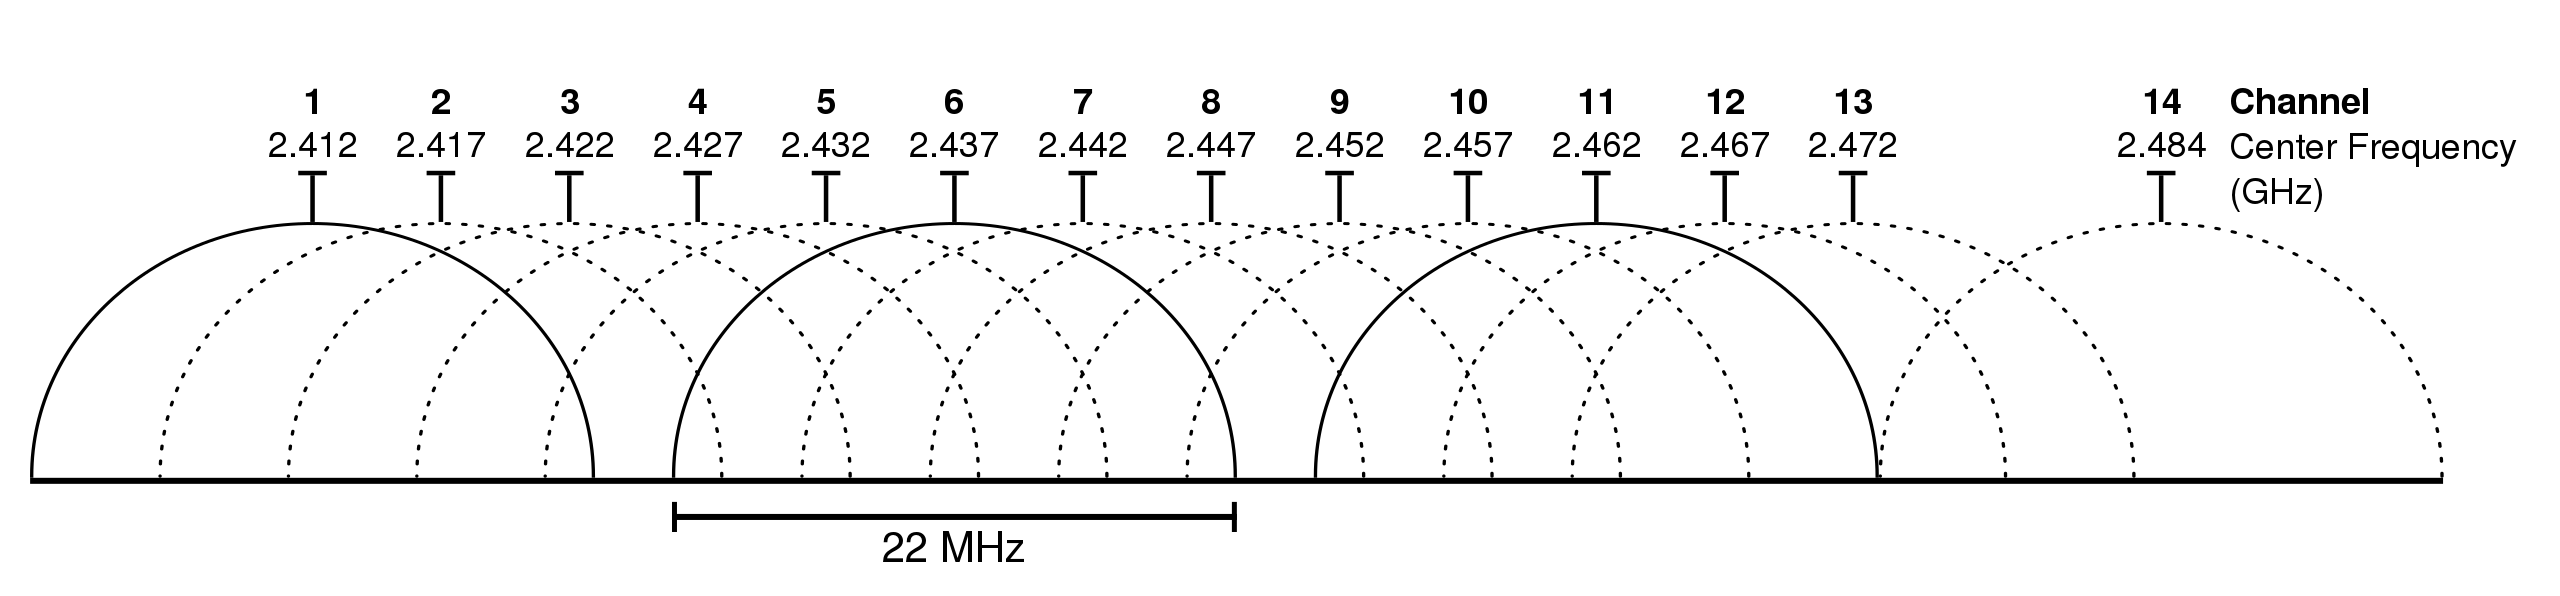
\includegraphics[width=0.75\textwidth]{images/wifi_channels.png}
    \end{figure}
    These channels specifically reside in an industrial, scientific and medical
    (ISM) band. This standard also provides datagram frames for the transport
    layer.
\end{flushleft}
\begin{flushleft}
    % TCP
    Transmission Control Protocol (TCP) will be used to satisfy transport layer
    requirements of the product, and will be used to transmit symbols (i.e.
    from any commands, data, settings, telemetry, etc.) between Amazon Web
    Services (AWS) and the microcontroller (MCU). TCP was chosen over other
    protocols, such as User Datagram Protocol (UDP), mainly due to its
    reliability. The extent of TCP's reliability includes features such as
    checksums, duplicate data detection, retrying of transmissions, sequencing,
    and timers.
    Such reliability is favored over higher bandwidth or lower
    latency, as neither of the latter are required for the kilobytes
    of information being relayed between AWS and the MCU. A standard TCP frame
    is shown in \autoref{tcp_frame}.
    \begin{figure}[H]
        \caption{TCP frame (\href{https://condor.depaul.edu/jkristof/technotes/tcp.html}{The Transmission Control Protocol}, Fig. 1)}
        \label{tcp_frame}
        \centering
        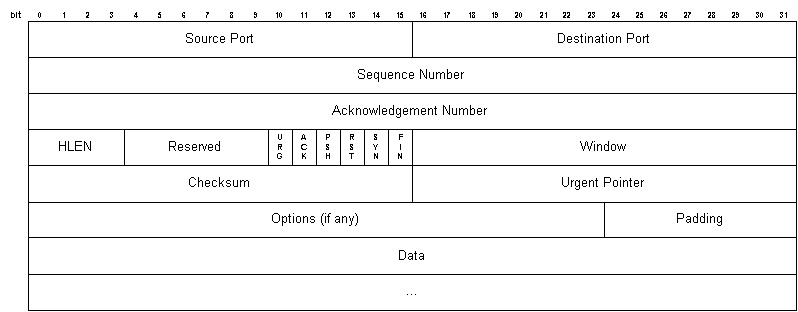
\includegraphics[width=0.75\textwidth]{images/tcp_frame.jpg}
    \end{figure}
\end{flushleft}        % Section 4.1 - what standards do we have to adhere to?
\subsection{Constraints}
The constraints discussed in the following subsections refer to limitations on the team's ability to design the system. Each section will discuss possible and realized problems with regard to the specific category of constraint. Following the discussion of the problem the team will discuss some possible or implemented solutions.
\subsubsection{Economic}
Although different sponsorship options were explored as a source of funding for our product, ultimately our team has not received any sponsorship for this product. This process will be entirely self-funded and evenly divided between the four team members. As a result of this, component selection heavily considers unit cost as a factor. It follows that the parts selected for this endeavor will meet the minimum requirements, but may not have some of the "nice-to-have" features one may want from a specific component. 
\subsubsection{Time}
When it comes to time constraints, this project is on a deadline. Most projects are on a deadline in order to ensure the customer can make full use of the project as ordered. In this case, the project is part of a larger organization that runs through business cycles every year. The deadline in place is imposed by the restructuring of the university as a workforce.

An additional time constraint is university leave. As a workforce, UCF mandates that work be suspended for certain occasions, including hurricanes, as we were recently reminded.

Our design process has revolved around flexibility, and as a result we have not been forced to wait in order to acquire the products we need to design our project. However, as the spring approaches and designs become finalized, we will lose this flexibility. 

\subsubsection{Equipment}
There are three main equipment constraints on our ability to produce our project. One is limited access to software, another is heavily shared tools, and the third is having facilities to build.

This project arises out of a tradition of problem solving that is used in educational facilities and industries all over the country. A chief part of the College of Engineering and Computer Science program is to teach students to use the tools industry uses to solve the problems industry faces. So far, our team has used multiple integrated development environments, version control platforms, word processers and file viewers, text, video and audio communication services, and software for designing optical beam paths, CAD models of physical structures, and PCB simulations in order to express and determine design features for our project. Each of us has had tools that we would like to have used, but could not, either because of licensing, inexperience, or the need to work cooperatively with the larger team. 

Another equipment constraint has been in the form of shared workspaces. In order to leverage these tools, we need relatively quiet space to sit where we can communicate with each other and run power hungry devices while connected to the internet and organizational networks. Our University has provided us with design labs, but their tools are managed by students, and inventory is often untraceable and disorganized. 

The third equipment constraint is unique to the nature of this project, but it comes from needing to build outdoors. Building a garden bed requires land, if only a little, and although parts can be fabricated in clean spaces the system is designed to contain wet, heterogeneous dirt. Space outdoors is necessary to build and that means either permission from the University or leveraging team member access to land. 

Each of these equipment constraints has a different effect on the project, some of them are easy to get around, by finding open source alternatives to licensed software, by cooperating with other students to get more out of leftover optical components, and by using student networks to determine where and when our group will have space to meet. Some are more difficult, causing us to trade time and money that we would rather not have had to give. In the end, equipment constraints will not likely impact the project deadline or affect the features as laid out in the document.

\subsubsection{Safety}
This project features several threats to human safety that must be addressed. The power subsystem is rated with sufficiently high voltage and current to cause cardiac arrest. The user must be protected from direct exposure to electrical conductors within the system, especially as this is an outdoor system with water management mechanisms which may add to the risk. The optical subsystem involves the use of infrared probes and focusing lenses. If handled carelessly, these could potentially create an eye hazard during testing or product use that the victim would not be able to detect. Steps must be taken to indicate the nature of the threat where it exists. Other risks involved in the project include the chance of a minor cut on a sharp surface becoming infected from exposure to the soil. The structure and components of the project must be sufficiently dull to ensure against the possibility of this. 

\subsubsection{Environmental}
This project features a garden bed, which means that it will be directly engaging with the environment. Potential risks to the environment include project placement disturbing existing ecosystems. This can occur through fertilizer runoff, sound pollution, light pollution, introducing invasive species, poisoning local wildlife, entrapping or injuring animals, or destruction of a natural resource part of the ecosystem relies on. Another environmental consideration is the effect this project will have on the environment through engaging human systems such as drawing on the city power and water supply. Our team hopes to use subsystems to mitigate and even eliminate these potential consequences.

\subsubsection{Manufacturability}
Manufacturability is a set of important criteria for early in the design process to avoid making costly mistakes. There are two reasons a design, once complete, might not be manufacturable. One, the design cannot feasibly be produced. Two, the cost of the design is prohibitive. Our team has protected against cost prohibitive manufacturability issues by ensuring that our component selection is traceable and that each component is in production and within our price range at cost, not due to clearance discounts. Another step our team is taking against future constraints is selecting the bulk of our components and design features before taking steps toward production.  

\subsubsection{Ethical}
Thankfully, our project makes use of institutions and practices that are well within the bounds of ethical behavior. Our garden bed will encourage age old activities that do not threaten the well being of the user or the surrounding community. Our project is designed to accommodate and minimize its environmental impact. Our use of wireless communication is extremely limited in its capability to cause harm to the user or to create a security risk for them or their neighbors. Users who engage with the product will not be able to use it to harm others, knowingly or unknowingly. The product does not in its nature risk damaging any cultural heritage or societies. Our team commits to submit to University policy as regards the goals and activities of this project.

\subsubsection{Sustainability}
Sustainability means creating a system that will produce as much of the resources as it uses so that the system does not collapse. This project does exactly that. The power generation subsystem is intended to ensure that our system does not need to draw on the power grid in order to function correctly. The water detection system is intended to ensure that water is not wasted reirrigating plants that have already been fed by the rain. In a broader sense, our project will increase the wellbeing of people’s lives, producing new plants and possibly food. One obstacle to sustainability is power storage. Our system uses a solar panel to collect energy, but that energy needs to be stored in order to distribute it in the right amounts and at the right times. 
 % Section 4.2-4.9 - what concerns are in the project?
\section{System Hardware and Software Design}   % Section 5 - how each section is going to work
\subsection{Controller Subsystem}
\label{sec:controller_subsystem}
\begin{figure}[H]
    \label{mcu_block_diagram}
    \caption{MCU block diagram}
    \centering
    % Need to update block diagram
    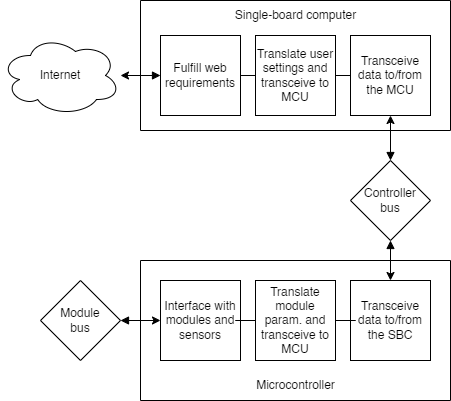
\includegraphics[width=0.75\textwidth]{images/mcu_block_diagram.png}
\end{figure}
% I need to write 11 pages lmfao
\begin{flushleft}
    % Why the MCU connects to the internet
    In order for our system to be as self-sufficient and power efficient as
    possible from an end-user perspective, it was determined that our system
    would require an internet connection to offload remote command-and-control
    to an Amazon Web Services EC2 instance (hence referred to as "AWS" and detailed in
    \autoref{sec:web_subsystem}). To make the process of operating our product 
    as hands-off as possible to end-users, the microcontroller will connect to
    the user's home WiFi network for access to AWS. Bluetooth, Zigbee, Thread,
    and other short-range 2.4 GHz communication protocols were disfavored over
    WiFi, as we predict most users will not have a device to dedicate to
    connecting our product via such protocols. Long range (LoRa) protocols were
    deemed unncessary, as the intended placement of our product is outside, 
    near or next to the user's home. We do not expect our product to produce
    or receive large amounts of data, so the decreased bandwidth of a
    WiFi-enabled product being beyond the outdoor walls of a building
    is not a significant drawback to our application. A wired connection
    (802.3/Ethernet) was deemed too invasive to the end-user. It is expected
    that most, if not all, end-users have a wireless access point and internet
    access. Thus, connection via the 802.11/WiFi standard was a natural choice
    for our use case.
    % maybe diagram of chip or network stack?
\end{flushleft}
\begin{flushleft}
    % How the MCU connects to the internet (local network, LAN -> NAT -> WAN,
    % TCP stack)
    The Texas Instruments CC3220-series of microcontrollers are WiFi-enabled
    chips with an ARM Cortex-M4 central processor and a WiFi network processor,
    along with many useful peripherals and power management modules. The WiFi
    network processor supports the following standards/features useful to our
    development:
    \begin{itemize}
        \item WiFi standards: 802.11b/g/n
        \item WiFi security: WEP, WPA/WPA2 PSK, WPA2 enterprise, WPA3 personal,
        WPA3 enterprise
        \item WiFi provisioning: SmartConfig, WPS2
        \item IP protocols: IPv4, IPv6
        \item IP addressing: static IP, DHCPv4, DHCPv6
        \item Transport: UDP, TCP, RAW
        \item Host interface: UART, SPI
        \item Built-in transceiver and 2.4 GHz antenna
    \end{itemize}
    Our microcontroller will 
    % WHAT KIND OF INTERFACE????
    % option a) web interface for user to long in to WLAN
    % option b) WPS button
    % don't forget IP addressing (most likely DHCP)
    % Interim: hardcode network login
\end{flushleft}
\begin{flushleft}
    % TCP sockets
    The MCU will communicate with AWS through TCP sockets. After connection to
    the user's home network, the MCU will check if there is an internet
    connection. Once an internet connection has been established, the MCU will
    open a socket and connect to the AWS instance via its URL (using the
    default DNS nameserver provided to network clients).
\end{flushleft}
\begin{flushleft}
    % Parameters for connection and how often it tries
    Once the MCU has established a connection to the internet and the AWS
    instance, it attempts to send current system settings and telemetry, as
    well as sensor readings to AWS. The microcontroller does this at least
    once every 15 minutes. Sending and receiving may occur more often if
    commanded to by AWS. Because TCP is being used to connect AWS and the
    microcontroller, any manual retries on a failed send or receive most
    likely will be futile. Therefore, any sort of link error handling will
    be performed by the link and not the microcontroller program.
\end{flushleft}
\begin{flushleft}
    % Any over-the-air updates?
    At this time, our team does not intend to provide a method for over-the-air
    updates (OTA), however, this is a provision that may be developed in the
    future.
\end{flushleft}
\begin{flushleft}
    % MCU receives commands, decodes commands
    The MCU will receive commands and data from AWS in the following form:
    \begin{center}
        \texttt{t x c y}
    \end{center}
    where \texttt{t} (character) marks the beginning of the command string,
    \texttt{x} (unsigned integer) indicates how many seconds to wait before
    executing command \texttt{c} (character) with parameter \texttt{y}
    (ambiguous). The following characters occupy the spot of \texttt{c}, and
    translate to the following commands:
    \begin{center}
        \texttt{w y}: water, \texttt{y} is boolean \\
        \texttt{a y}: solar $\theta$, \texttt{y} is double \\
        \texttt{b y}: solar $\phi$, \texttt{y} is double \\
        \texttt{l y}: low power, \texttt{y} is unsigned int for flags \\
        \texttt{s y}: send data, \texttt{y} is unsigned int for flags
    \end{center}
    For example, if AWS instructs the MCU to turn on the water source in 3
    minutes, it would send the command \texttt{t 180 w 1}. If AWS would like
    the MCU to change the $\theta$ of the solar panels to 45$\degree$
    immediately, it would send \texttt{t 0 a 45.0}. It is important to note
    that the values of \texttt{x} and \texttt{y} are not strings (e.g.
    45$\degree$ will not be sent as \texttt{"45.0"}), but the actual encoding
    of 45$\degree$ as a double-precision float. This is to maintain a
    consistent command string size amongst all transmissions.
    \begin{figure}[H]
        \label{command_bitwise}
        \caption{Bitwise representation of command}
        \centering
        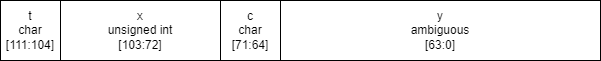
\includegraphics[width=0.75\textwidth]{images/command_encoding.png}
    \end{figure}
\end{flushleft}
\begin{flushleft}
    % Will program in C++. Any libraries, multithreading?
    % Singleton Pattern Thread for scheduling tasks
    It should be expected that all headers from the C++ standard library (as
    defined in C++23) will be used, along with the following nonstandard
    libraries: Texas Instruments SimpleLink™ CC32xx SDK. Additionally, it is
    expected that the MCU program will schedule tasks using a Singleton Pattern
    thread to ensure thread safety when accessing variables.
\end{flushleft}
\begin{flushleft}
    % Classes and class diagram
    There will be a few classes defined in the MCU's programming.
    %\begin{figure}[H]
        %\label{classes_uml}
        %\caption{UML diagram of the classes used}
        %\centering
        %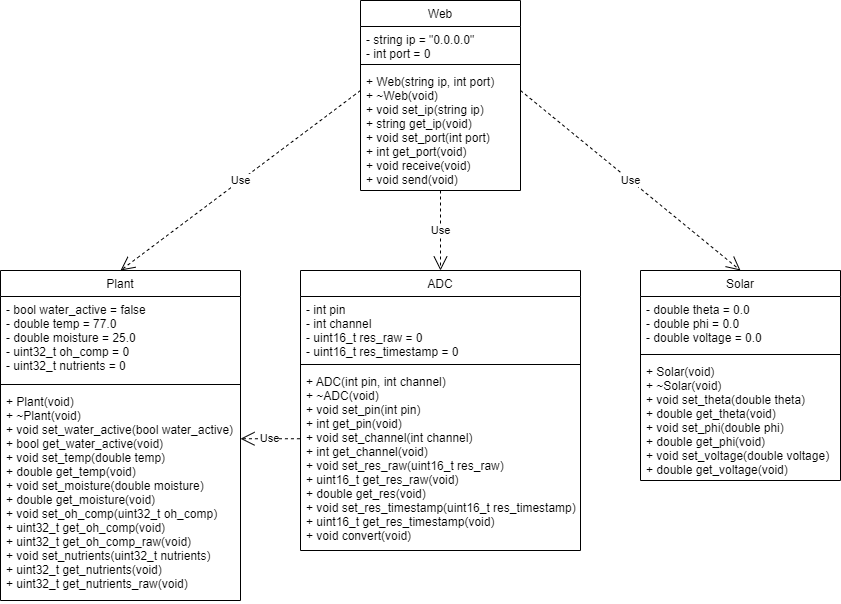
\includegraphics[width=0.75\textwidth]{images/classes_uml.png}
    %\end{figure}
    Classes will be laid out in a header file using the following defintions:
    \begin{flushleft}
        \texttt{class Plant \{}  \\
        \quad\texttt{private:} \\
        \quad\quad\texttt{bool water\_active;} \\
        \quad\quad\texttt{double temp;} \\
        \quad\quad\texttt{double moisture;} \\
        \quad\quad\texttt{uint32\_t oh\_comp;} \\
        \quad\quad\texttt{uint32\_t nutrients;} \\
        \quad\texttt{public:} \\
        \quad\quad\texttt{Plant();} \\
        \quad\quad\texttt{set\_water\_active();} \\
        \quad\quad\texttt{get\_water\_active();} \\
        \quad\quad\texttt{set\_temp();} \\
        \quad\quad\texttt{get\_temp();} \\
        \quad\quad\texttt{set\_moisture();} \\
        \quad\quad\texttt{get\_moisture();} \\
        \quad\quad\texttt{set\_oh\_comp();} \\
        \quad\quad\texttt{get\_oh\_comp();} \\
        \quad\quad\texttt{set\_nutrients();} \\
        \quad\quad\texttt{get\_nutrients();} \\
        \texttt{\};} \\
    \end{flushleft}
    \begin{flushleft}
        \texttt{class Solar \{}  \\
        \quad\texttt{private:} \\
        \quad\quad\texttt{double theta;} \\
        \quad\quad\texttt{double phi;} \\
        \quad\quad\texttt{double voltage;} \\
        \quad\texttt{public:} \\
        \quad\quad\texttt{Solar();} \\
        \quad\quad\texttt{set\_theta();} \\
        \quad\quad\texttt{get\_theta();} \\
        \quad\quad\texttt{set\_phi();} \\
        \quad\quad\texttt{get\_phi();} \\
        \quad\quad\texttt{set\_voltage();} \\
        \quad\quad\texttt{get\_voltage();} \\
        \texttt{\};} \\
    \end{flushleft}
    \begin{flushleft}
        \texttt{class Web \{}  \\
        \quad\texttt{private:} \\
        \quad\quad\texttt{string ip;} \\
        \quad\quad\texttt{int port;} \\
        \quad\texttt{public:} \\
        \quad\quad\texttt{Web();} \\
        \quad\quad\texttt{set\_ip();} \\
        \quad\quad\texttt{get\_ip();} \\
        \quad\quad\texttt{set\_port();} \\
        \quad\quad\texttt{get\_port();} \\
        \texttt{\};} \\
    \end{flushleft}

    % Turn structs into classes
    % Get rid of telemetry
    % Implement default state

    % Structs (or maybe classes):
    %  Water
    %  Solar
    %  Battery/charge controller
    %  AWS/socket
    %  Telemetry (own system)
\end{flushleft}
\begin{flushleft}
    % Send to AWS, format and types of commands
    % Send straight data from the struct
    No data that would be exclusively considered telemetry will be transmitted 
    between AWS and the MCU (e.g. processor temperature). Instead, all
    "telemetry" values will be handled with interrupts and ISRs/functions
    on-chip, while current settings and sensor readings will be transmitted
    back to AWS.
\end{flushleft}
\begin{flushleft}
    % Global vars
    No global variables plan to be implemented at this time.
\end{flushleft}
\begin{flushleft}
    % Functions
\end{flushleft}
\begin{flushleft}
    % Interrupts and ISRs
    If the charge controller indicates that the battery has fallen below a
    certain voltage (named "low voltage"), the MCU will raise an interrupt and
    execute \texttt{isr\_low\_power()}. This ISR performs housekeeping before
    putting the MCU into a low power state, limiting use of its functions.
\end{flushleft}
\begin{flushleft}
    % Interrupts and ISRs (cont.)
    If the charge controller indicates that the battery has fallen below a
    certain voltage (named "critical voltage"), the MCU will raise an interrupt
    and execute \texttt{isr\_critical\_power()}. This ISR performs further 
    housekeeping before putting the MCU into an extreme low power state,
    limiting all but the features necessary to maintain a connection with AWS.
\end{flushleft}
\begin{flushleft}
    % Interrupts and ISRs (cont.)
    If the MCU, AWS, or any other devices transmit indication of a dangerous
    state or if the MCU, AWS, or any other devices transmit indication of a
    shut down the MCU will raise an interrupt and execute
    \texttt{isr\_shut\_down()}. This ISR immediately shuts down all able
    subsystems, and puts all other subsystems in a fail safe state. This ISR
    fails safe the entire system.
\end{flushleft}
\begin{flushleft}
    % Interrupts and ISRs (cont.)
    If the MCU receives indication of a start up (via a momentary switch), the
    MCU will raise an interrupt and execute \texttt{isr\_start\_up()}. This ISR
    starts up all relevant subsystems and begins the MCU's programming. This
    ISR starts up the entire system.
\end{flushleft}
\begin{flushleft}
    % File organization (main, header files, other source files, etc.)
\end{flushleft}
\begin{flushleft}
    % How the MCU gets data from sensors (ADC)
\end{flushleft}
\begin{flushleft}
    % How MCU sends data to servos
\end{flushleft}
\begin{flushleft}
    % What sort of telemetry we'll have
    % No telemetry
\end{flushleft}
\begin{flushleft}
    % What kind of development model?
    % Probably agile
    An Agile development model will be used.
\end{flushleft}
\begin{flushleft}
    % IDE and Git
    Texas Instruments Code Composer Studio v12 will be used to program,
    compile (via TI ARM compiler v20), and debug the C++-based project. GitHub
    will be used as a repository for the project, using Git for version
    control.
\end{flushleft}                  % Section 5.1 
\subsection{Power Subsystem}
\label{sec:power_subsystem}
The power system is an important part to any electrical device or component that requires any amount of power. Most often, it starts from a power source such as a battery or wall outlet then is converted into energy to operate what is being used. At the minimum, this model is designed to be an independent system, having the capability to operate on its own. The way that can be achieved is through solar power. \par
Solar power has been such a strong growing source of energy and will play a vital role in our system. Power is collected through the solar panels and then regulated through the charge controller to ensure that the battery is receiving the correct amount of charge. The power is regulated through the charge controller so that the battery is not being over charge, which could potentially damage it and reduce the battery life in the future. It is then stored in a battery when the system is not operating and then utilized when needed. From there, voltage needs to be regulated again throught the voltage regulator for the microcontroller and other components that require different amounts of voltage. The block diagram in \autoref{fig:power-block-diagram} shows the flow of power through the system. 

\begin{figure}[H]
    \centering
    \caption{Power subsystem block diagram}
    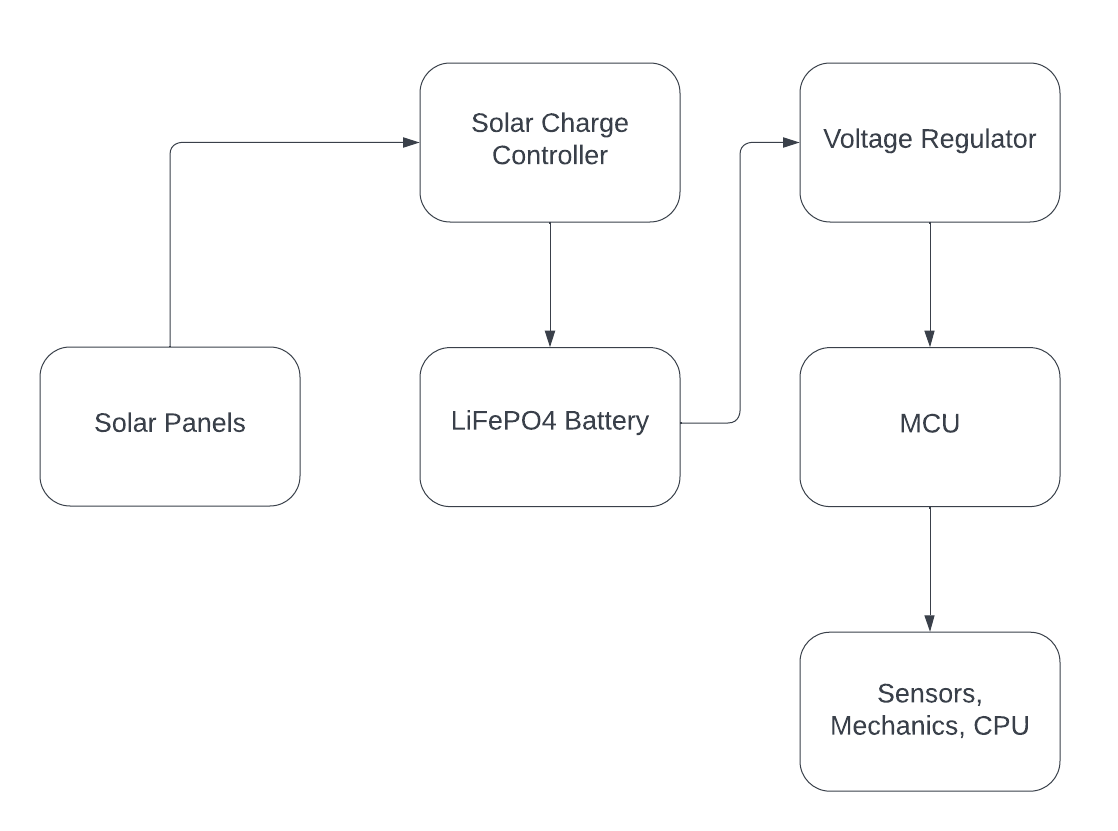
\includegraphics[width=\textwidth]{images/Power_System_Flowchart.png}
    \label{fig:power-block-diagram}
\end{figure}
The block labeled ``Mechanics'' in \autoref{fig:power-block-diagram} refers to the solenoid valve for controlling water flow as well as the control scheme for actuating the solar panels to maximize power efficiency.
\subsubsection{Solar Panel Control}
To get a greater degree of accuracy the use of stepper motors are used. First, based on the choice of solar panels we get the mass and dimensions of the solar panels, these are .76kg and .336m x .2m respectively. This is important for calculating the torque. We only need to provide two degrees of freedom, one about the short axis (the horizontal axis that bisects the .2m side) and the vertical axis (the axis at the intersection that bisects the two sides of the panel). From the length and mass we can calculate the force per unit length:
\begin{equation}
    \frac{.76 \text{kg}}{.336 \text{m}}=22.62\frac{\text{N}}{\text{m}}
    \label{eqn:short-axis-fpl}
\end{equation}
Now, knowing that torque is $F\times d$ we can formulate the torque for any given angle about this axis in the following:
\begin{equation}
    \int_{0}^{.168} 22.62 \times x \times \sin{\theta} \, dx
    \label{eqn:short-axis-torque}
\end{equation}
\autoref{eqn:short-axis-torque} gives the torque for any given angle. Something you might have noticed is that this is for only one side of the panel. The full torque about the central axis is as follows:
\begin{equation}
    \int_{0}^{.168} 22.62 \times x \times \sin{\theta} \, dx - \int_{0}^{.168} 22.62 \times x \times \sin{180-\theta} \, dx
    \label{eqn:short-axis-torque-total}
\end{equation}
From \autoref{eqn:short-axis-torque-total} we can find the maximum and minimum values of the torque about the axis by finding the crossings of the first derivative with respect to $\theta$ and finding the concavity in the second derivate with respect to $\theta$. Doing so proves the intuition that there is no torque around either axis, this equation evaluates to 0 for all $\theta$.

To save on power \autoref{fig:stepper-config} shows that two motors will work to rotate the panels about the short axis while the center axis is actuated by a single motor and belt system.
\begin{figure}[H]
    \centering
    \caption{Stepper motor configuration}
    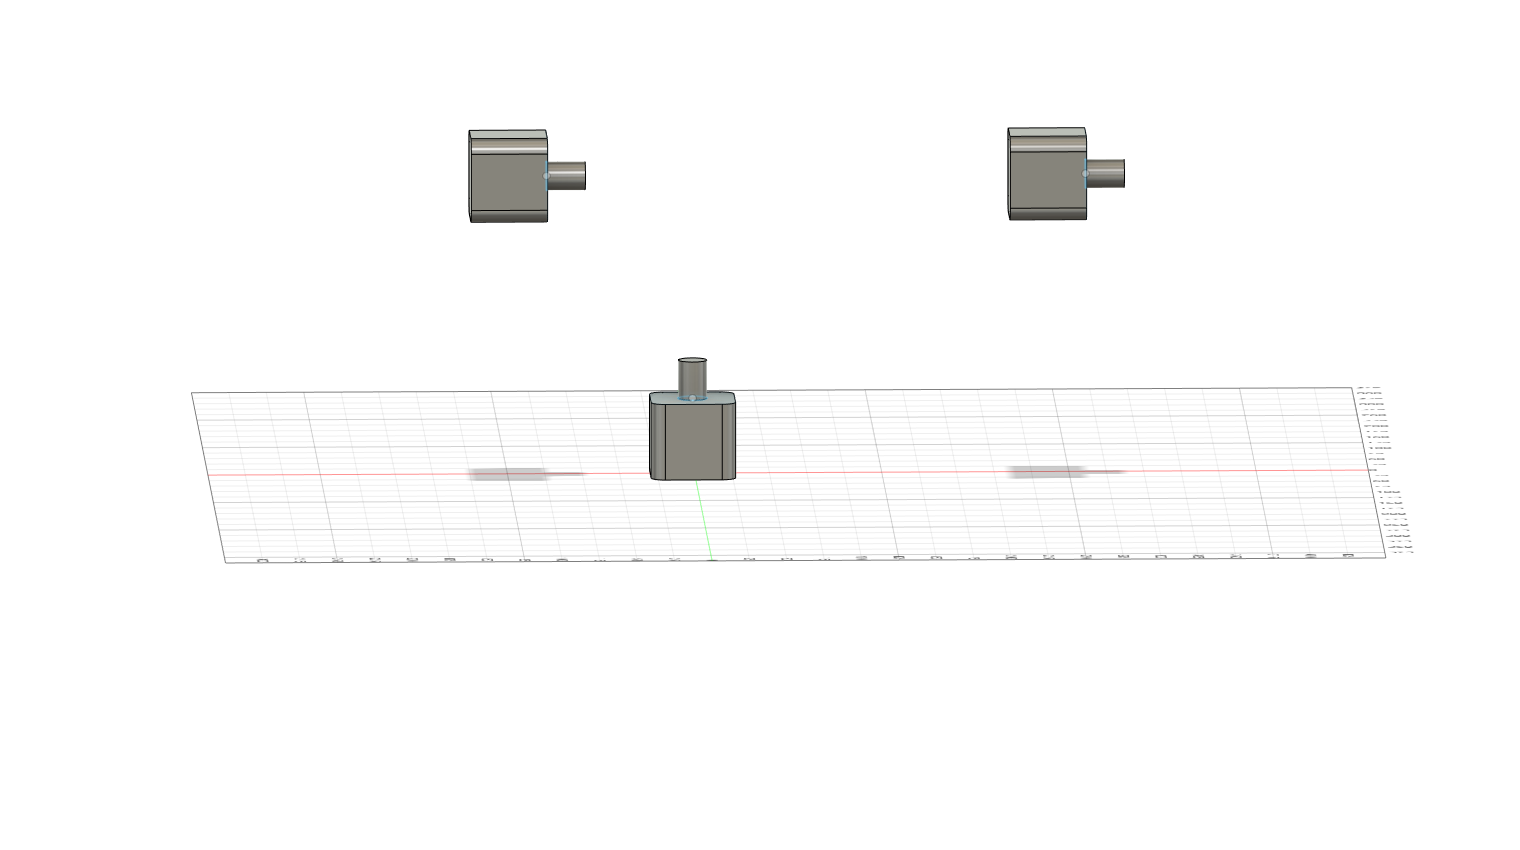
\includegraphics[width=0.5\textwidth]{images/stepper-config.png}
    \label{fig:stepper-config}
\end{figure}
The reason we have to use two stepper motors for the short axis rotation is that because as the panels rotate about their central axis any rod or pulley or tensioner system would come out of alignment. Another advantage of this due to the lack of torque in the system is that using a motor controller the two motors can be driven with a single H-bridge with a minimum penalty to power, this will ensure that both panels are always pointed at the same angle in the desired direction.\par
\subsubsection{Voltage Regulator Designs}
As mentioned before, voltage regulators play an important role in regulating voltage throughout the whole model. They make sure that all the components like the microcontroller, sensors, mechanics, etc. are receiving the right amount of voltage.\par
The CC3220 requires 3.3V to operate and the sensors will be running on 5V. With the battery running at 12V, we would use the voltage regulator to supply the right voltage amount to each component. To perform and achieve the proper regulation, we created different design schematics for the LM317 (Linear) voltage regulator and the LM2576 (Switching) regulator. Along with that, we created DC/DC designs on WEBENCH as a consideration for specific conditions.\par
\paragraph{Linear Voltage Regulator Designs}
The linear voltage regulator schematic was designed to generate an output voltage of 3.3V for the CC3220. This circuit schematic is obtained from the LM317 voltage regulator datasheet, Figure 39, and then designed on Multisim with capacitors, resistors, and diodes. From the datasheet, there were values that were given and from there we had to find values and then test them. The CADJ we used 1uF as a constant and then 390Ω was used for the value R. With these inputed values, we achieved an estimated 3.3V and measuring the adjustment current we got 5.2634mA as shown in Figure 40.\par
\begin{figure}[H]
    \centering
    \caption{LM317 Linear Voltage Regulator }
    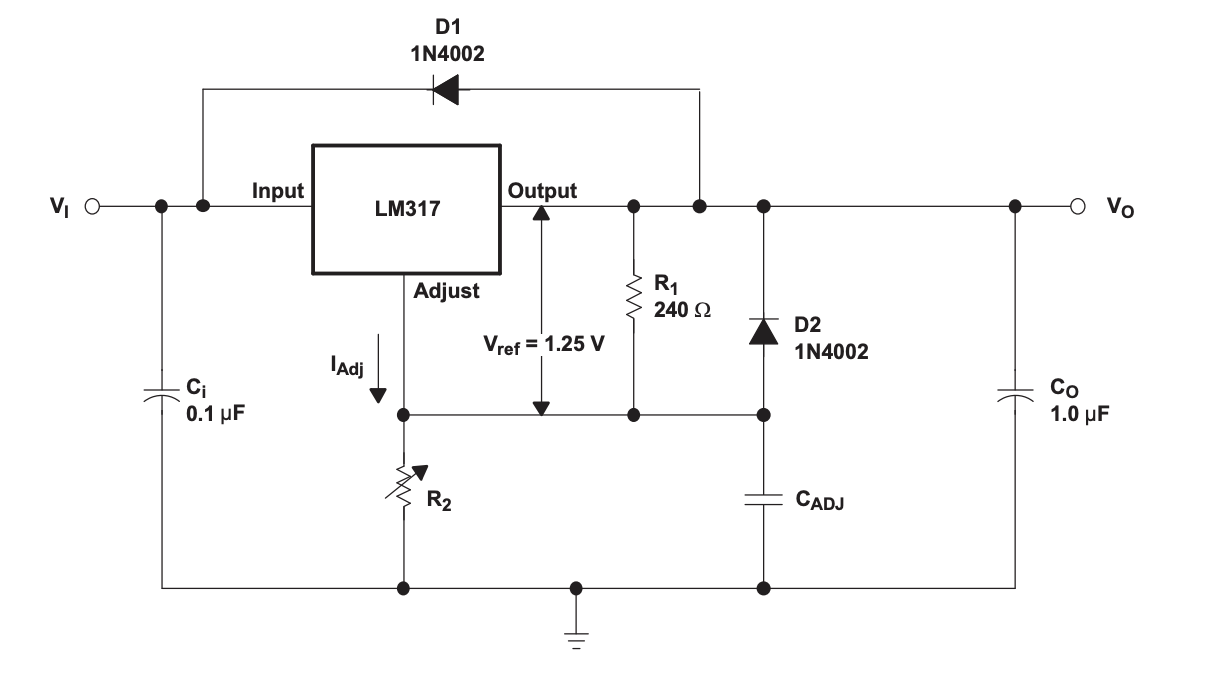
\includegraphics[width=\textwidth]{images/LM317_Application_schematic.png}
    \label{fig:linear-voltage-regulator}
\end{figure}
\begin{figure}[H]
    \centering
    \caption{LM317 3.3V Linear Voltage Regulator}
    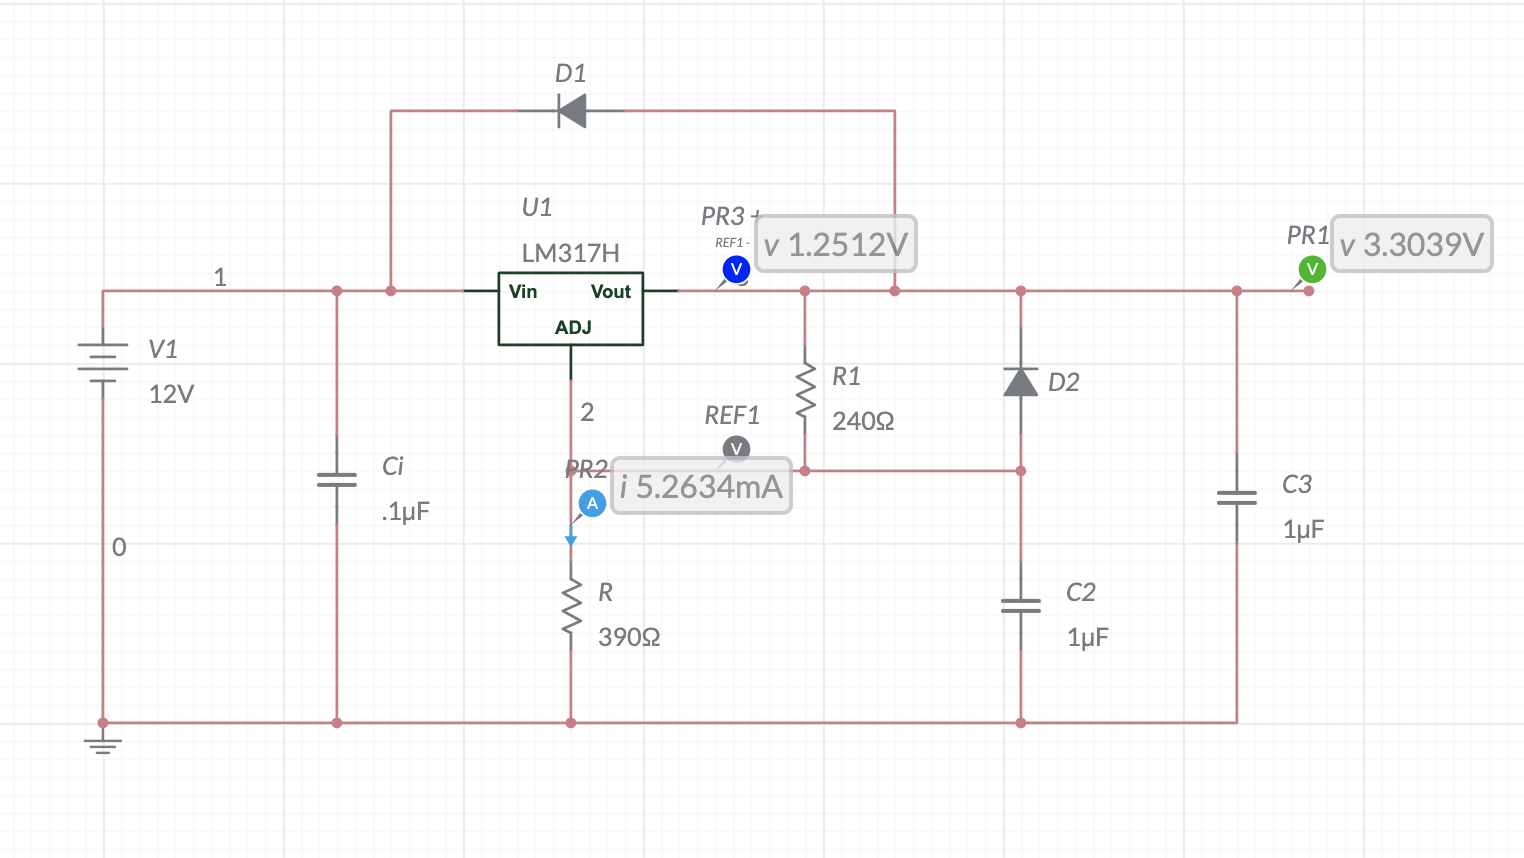
\includegraphics[width=\textwidth]{images/LM317_3.3_schematic.png}
    \label{fig:3.3V-linear-voltage-regulator}
\end{figure}

In Figure 41, we re-designed the ciruit get the regulated output voltage of approximately 5V for the sensors. This is done with the same circuit as for the 3.3 output voltage regulation, but the value R is now 720Ω with CADJ still remaining at 1uF. With these values that we found we achieved an output voltage of about 5V and the adjustment current of 5.2617mA.\par
\begin{figure}[H]
    \centering
    \caption{LM317 5V Linear Voltage Regulator}
    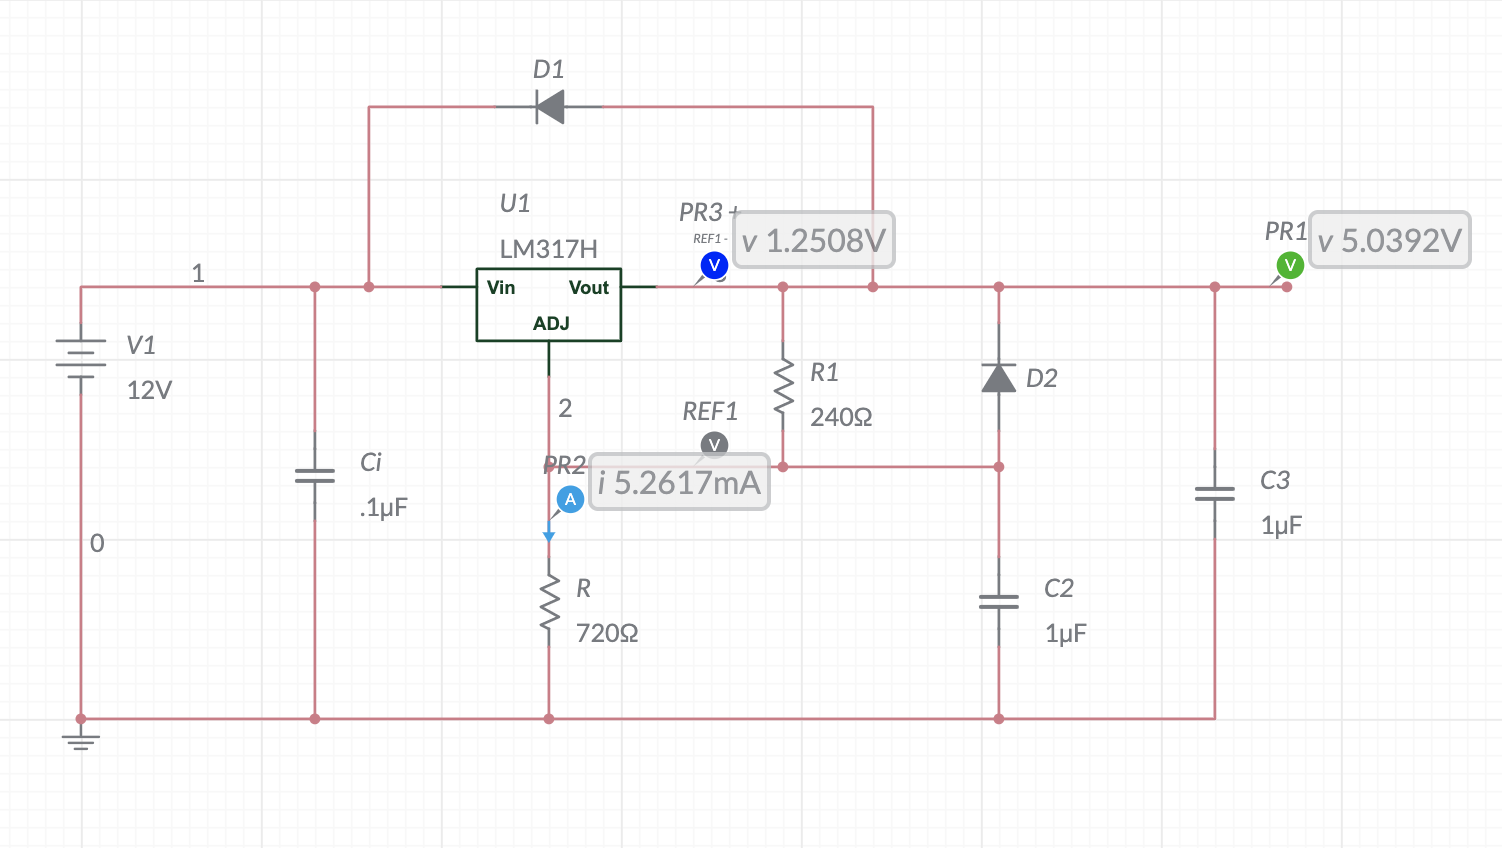
\includegraphics[width=\textwidth]{images/LM317_5_schematic.png}
    \label{fig:5V-linear-voltage-regulator}
\end{figure}
\paragraph{}In this testing, we were able to verify that the LM317 Linear voltage regulator can output the proper voltages. Along with this testing, we also went ahead to see if the voltage regulator was able to output higher voltage levels. For this testing we wanted to see if we could achieve a regulated output voltage of 12V. Using the same circuit for the output voltages 3.3V and 5V, we changed the value of R to increase the output voltage. We were unable to get the regulated 12V from the output. Instead, the highest that it went up to was about less than 11V. During this test though, we noticed that when we past 2kΩ the adjusttment current and the voltage reference started to decrease. Not only that but the output voltage stayed between 10V and 11V, but didn't go higher than 11V.
\begin{figure}[H]
    \centering
    \caption{LM317 10V Linear Voltage Regulator}
    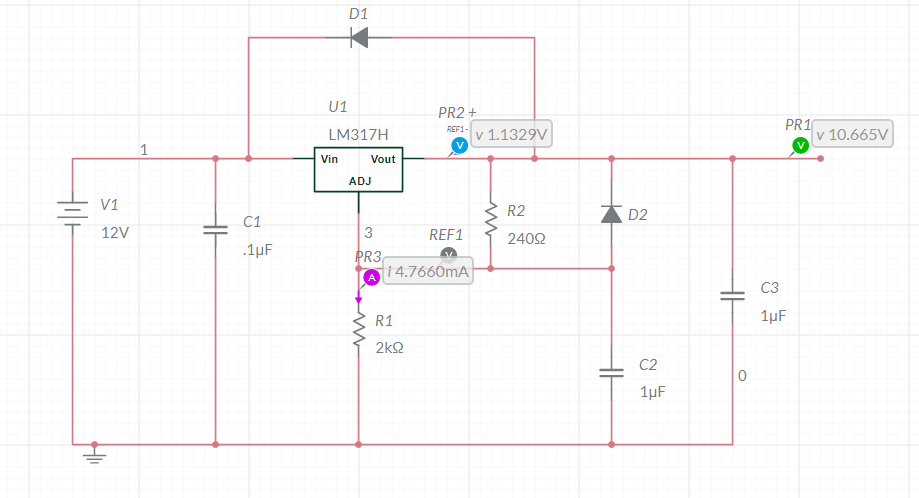
\includegraphics[width=\textwidth]{images/LM317_10_schematic.png}
    \label{fig:10V-linear-voltage-regulator}
\end{figure}
\paragraph{Switching Voltage Regulator Designs}
The same approach was used for the switching voltage regulator to find out how to achieve the correct output voltage. This will be done for the CC3220 microcontroller that operates at 3.3V and the sensors operating at 5V. Luckily, in the Texas Instrument datasheet they had schematic done for their fixed version as well as their adjustable version. In the fixed version, we are able to set the output regulated voltages to different amounts, such as 3.3, 5, 12, and 15V, leaving the load current fixed to 3A. This is shown in the figure below.\par
\begin{figure}[H]
    \centering
    \caption{LM2576 Fixed Switching Voltage Regulator}
    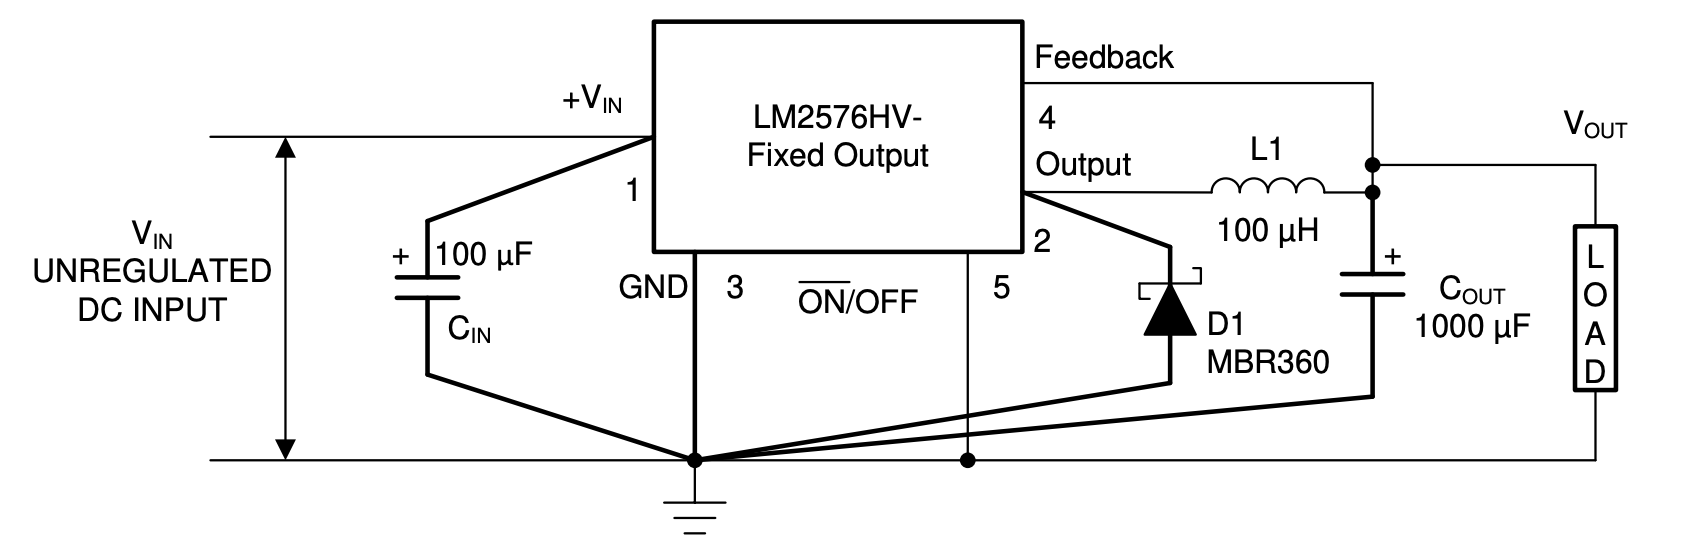
\includegraphics[width=\textwidth]{images/LM2576_Fixed.png}
    \label{fig:fixed-switching-voltage-regulator}
\end{figure}
For the adjustable version of the LM2576 switching voltage regulator, because it is adjustable, the maximum input voltage that is allowed by this version is 25V. The output regulated voltage can also only output 10V, maximum, with a constant load current of 3A, similar to the fixed version. This is shown in Figure 42. In this version as well we can see that values R1 and R2, on the right, need to be found to find the Vout. This can be done with the equations below as well.\par
\begin{figure}[H]
    \centering
    \caption{LM317 adjustable switching Voltage Regulator}
    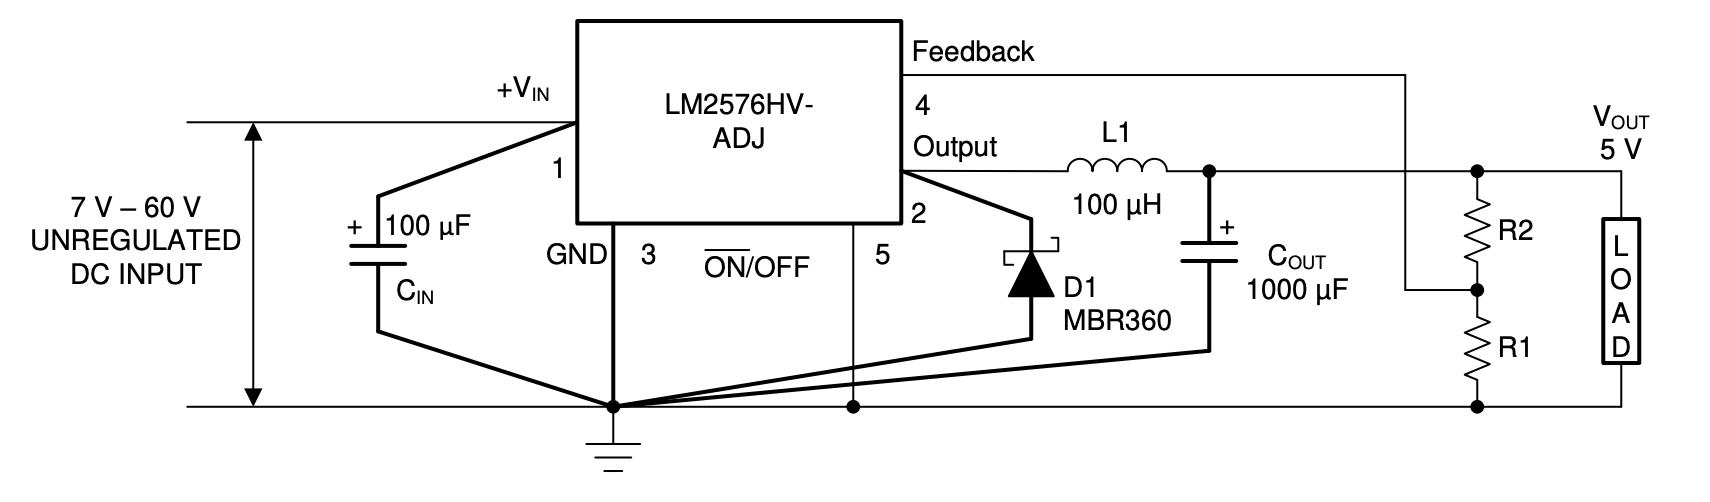
\includegraphics[width=\textwidth]{images/LM2576_Adjustable.png}
    \label{fig:5V-linear-voltage-regulator}
\end{figure}

\begin{figure}[H]
    \centering
    \caption{Switching Voltage Regulator Equations}
    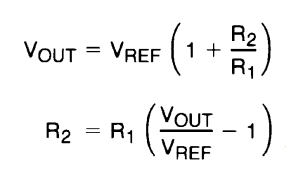
\includegraphics[width=\textwidth]{images/LM2576_Adjustable_equations.png}
    \label{fig:switching-voltage-regulator-equations}
\end{figure}
For this adjustable version, there is obviously no fixed value that the output voltage has to be. In this case, let's say the minimum outpute voltage of 10V We would still need to find the value in for 4 and the regulator chosen for. \par
 \paragraph{WEBENCH Designs}
 WEBENCH is a resource by Texas Instruments that helps design power supplies easily. This resource can be used for DC/DC power systems and AC/DC power systems. It is customizable and helps create various power supply circuits. In this software, we have the freedom to pick and choose our input and output values, and also consider if we want the desired circuit to be balanced, low cost, have high efficiency, or have a small footprint. \par
 For this system, we used input values between 8V and 22V and then output values of 3.3V with max current of 3A. With this we were able to find TPS62933, a high-efficiency, wide input range buck converter that is easy to use. This design itself provides an efficiency of 86.5\%, a BOM cost of \$1.34, and footprint of $195mm^2$. This is one of their low cost designs.\par
 \begin{figure}[H]
    \centering
    \caption{TPS62933}
    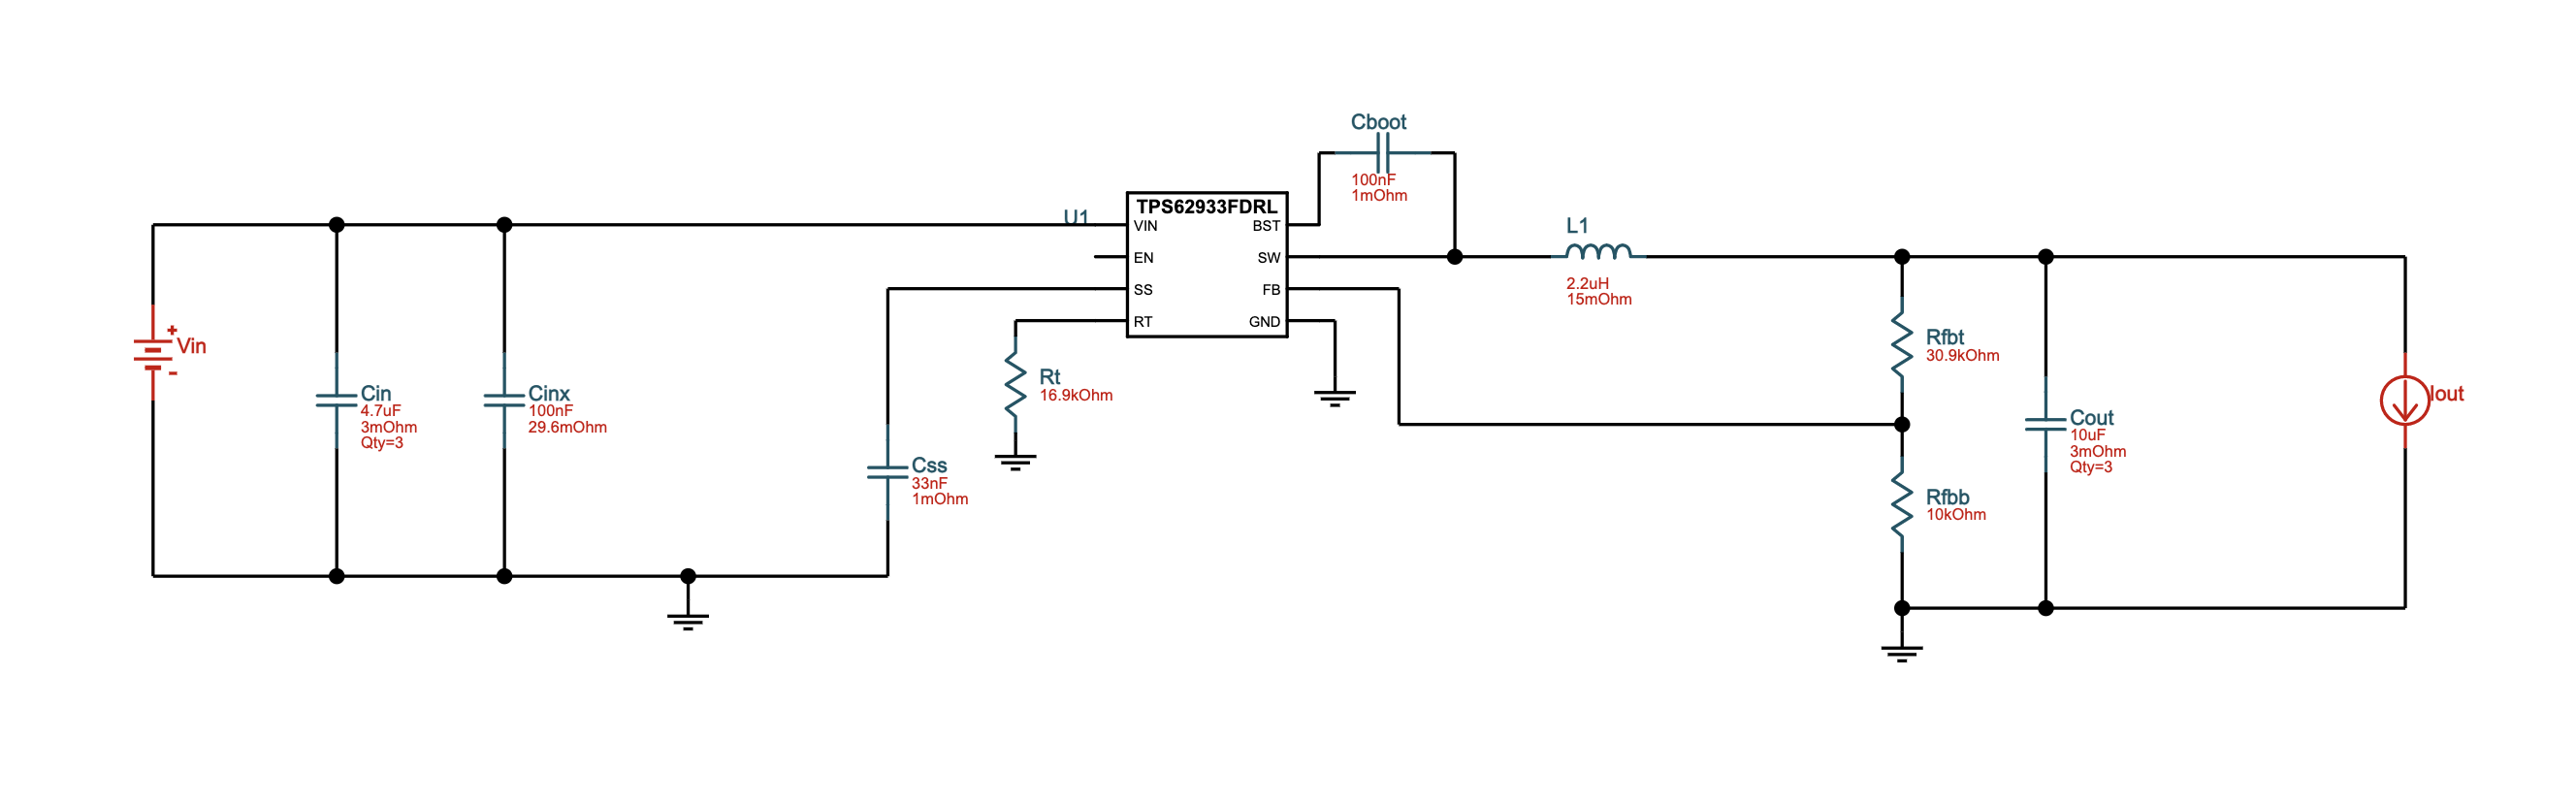
\includegraphics[width=\textwidth]{images/TPS62933.png}
    \label{fig:WEBENCH Design TPS62933}
\end{figure}
For the output regulated voltage 5V, the TPS62933 is also compatible for the 5V output regulation. Going back and changing the output value to 5V and changing the desired circuit consideration to a balanced circuit we find the TPS563300. This is also a high-efficient, easy-to-use buck converter that has a wide input range of 3.8V to 28V, but also supports an output current of 3A and regulates .8V up to 22V. The TPS563300 provides an efficiency of 91.5\%, a BOM of \$1.42, but a footprint of $516mm^2$. \par
\begin{figure}[H]
    \centering
    \caption{TPS563300}
    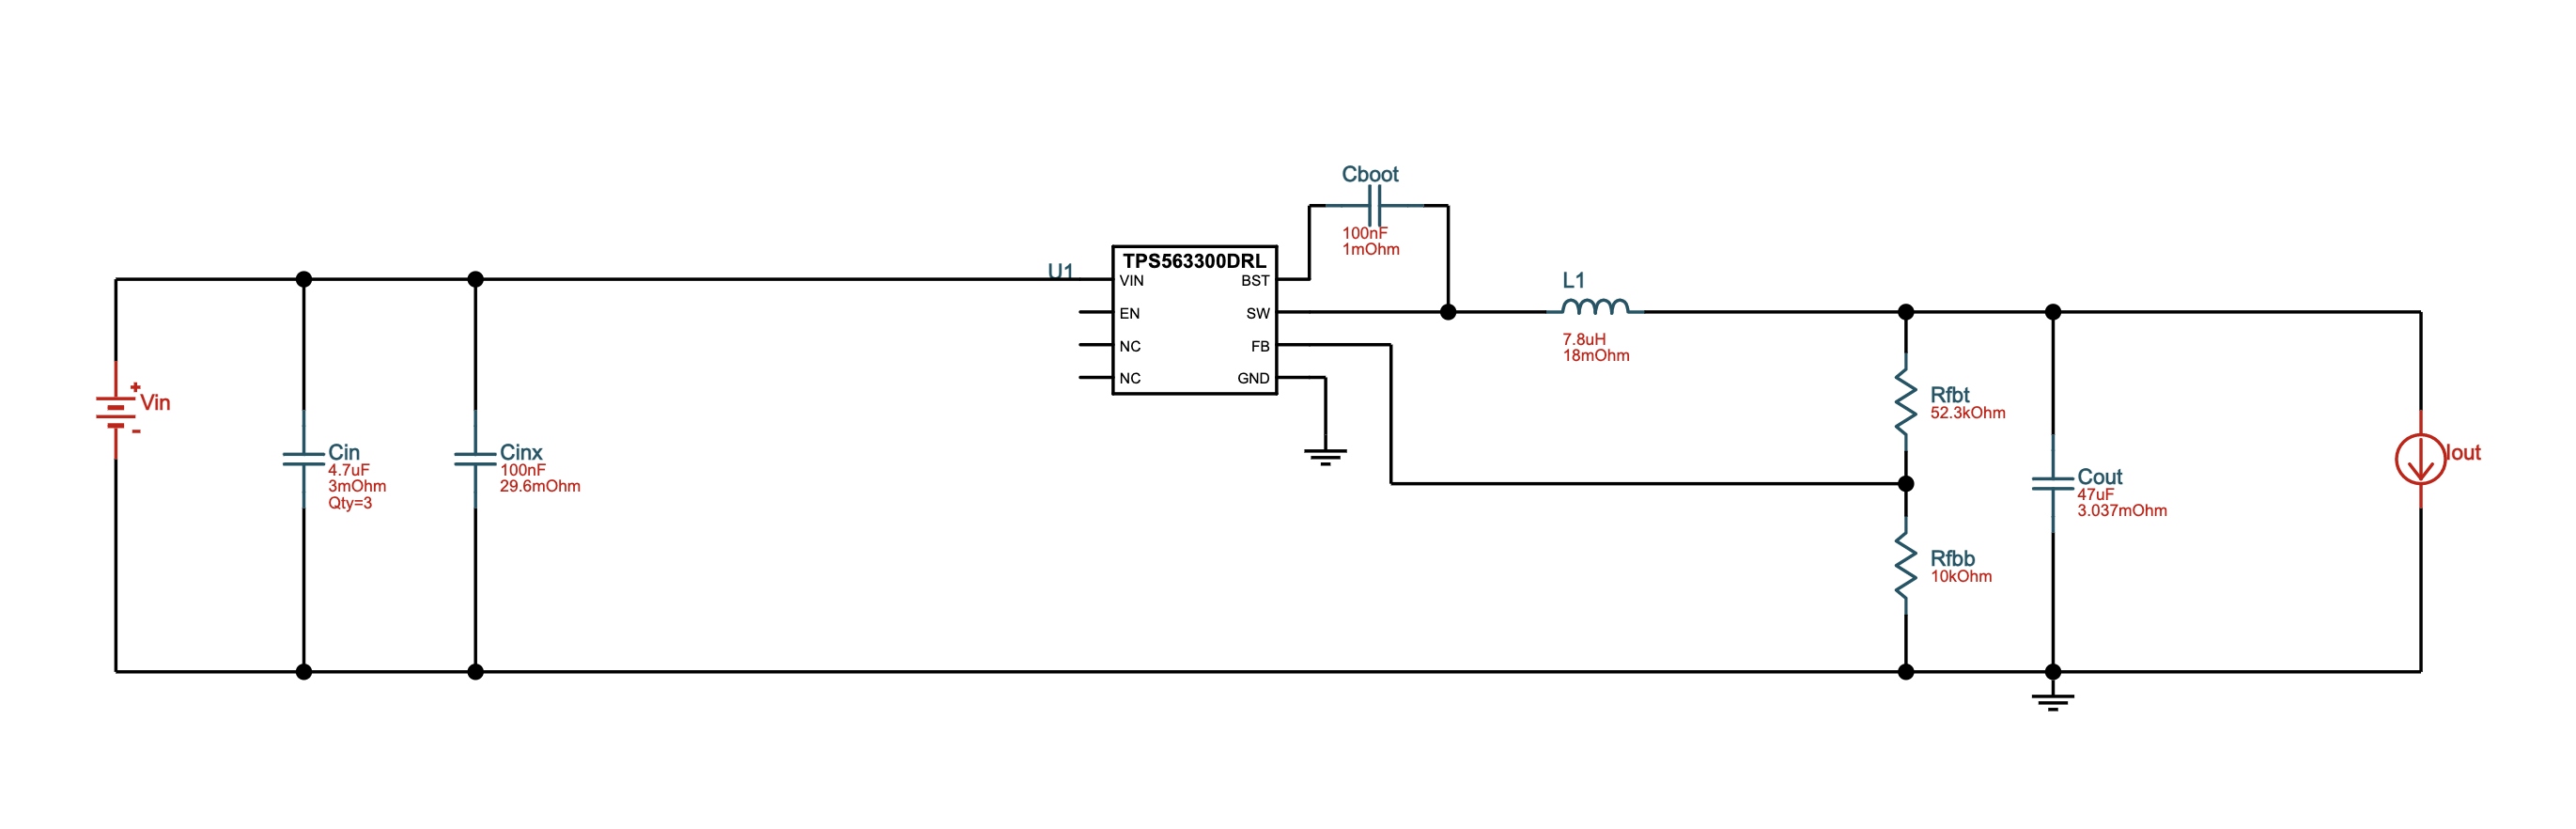
\includegraphics[width=\textwidth]{images/TPS563300.png}
    \label{fig:WEBENCH Design TPS563300}
\end{figure}
Although the TPS563300 is bigger, the price for the high efficiency this design provided would have been very good. It also doesn’t have that many other electrical components compared to the TPS62933, which adds to why it is easy-to-use.\par
After we are able to get all of the parts and components for the designed voltage regulators circuits, we can start testing each of them to see if the regulators are giving the proper output voltage and current that we theoretically found.\par                % Section 5.2
\subsection{Sensing Subsystem}
\begin{figure}[H]
    \caption{Sensing subsystem block diagram}
    \centering
    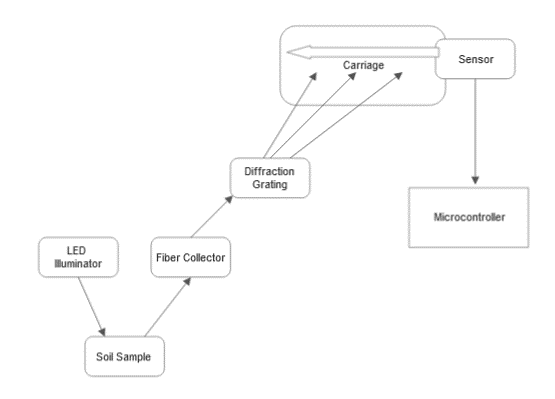
\includegraphics[width=0.75\textwidth]{images/OpticsBlockDiagram.png}
\end{figure}


The sensing subsystem is an infrared spectrometer that uses two photodiodes as detectors, a diffraction grating as a spectral separator, an array of LEDs to illuminate the target area, and optics to collect, collimate, and focus the beam. In order to determine the component positions and interaction, each component will have to be addressed.
    \begin{itemize}
        \item Ground
        \item LEDs
        \item Fiber in
        \item Fiber out collimated
        \item Reflective Diffraction Grating
        \item Focusing Lens
        \item Carriage driven Photodiodes
    \end{itemize}


    Dirt

That’s right, the first part of the optical subsystem is the soil. Structures in the soil emit trace electromagnetic signals that correspond to the soil matrix, soil temperature, soil moisture, and chemical content of the soil. (Link papers)
In order to ensure sufficient signal to noise ratio, the dirt is going to have to be probed by a bright, broadband source covering the visible and Near Infrared regime. Halogen lamps will do (link papers) but it may be possible to achieve the same effect with LEDs near the surface. 
An additional concern is that irregularities in the soil topography may reflect back light that would otherwise indicate organic components or water. In order to counter this, it is going to be necessary to flatten the dirt with a stamp or roller.


   LEDs

Placeholder until followup with ocean insight.

    Fiber in

placeholder

    Fiber out collimated

The fiber collimator selection hasn’t been finalized yet, but for now I’m assuming a beam of about 2mm diameter will come out of the fiber head collimated toward the grating.

    Grating

    The grating will be a 1200 groove per mm aluminum coating 1000nm blazed reflection grating. 
 
The grating equation governs the angle at which light of different frequencies will reflect. 
The first three orders of diffraction are plotted below for a 1200 groove per mm grating. The polar plot is degrees, ranging from 400nm to 1700nm. Rho represents the order of diffraction.
An angle of incidence of 45 degrees will produce backreflection toward the fiber collimator, however an angle of incidence at 50 degrees will not.

    Focusing Lens

    Carriage driven Photodiodes

    


\begin{figure}[H]
    \caption{Diffraction angle calculation}
    \centering
    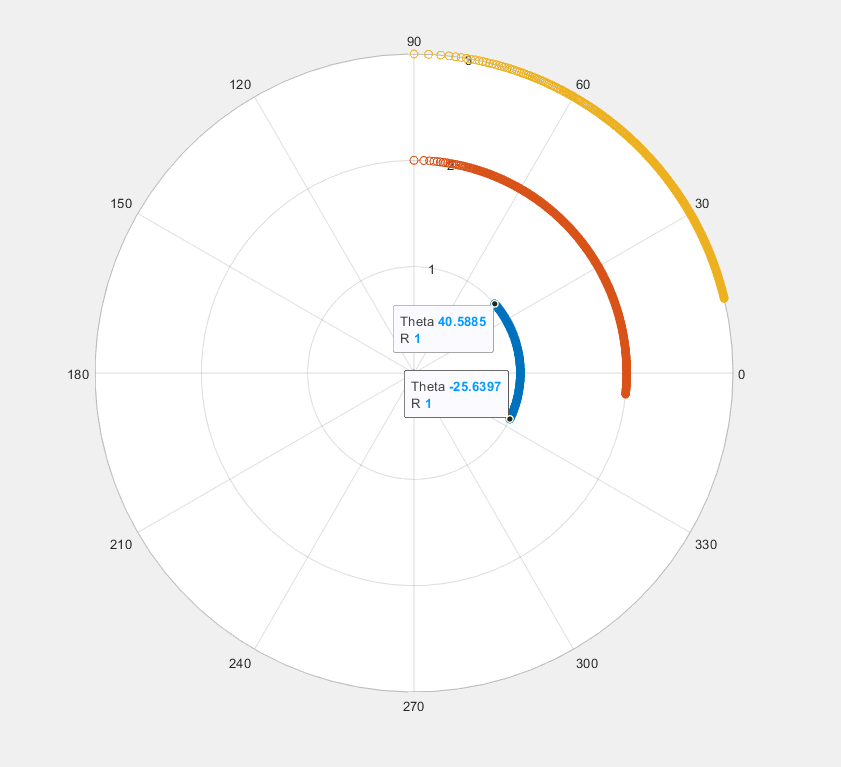
\includegraphics[width=0.75\textwidth]{images/DiffractionAngleCalculator.png}
\end{figure}

\begin{figure}[H]
    \caption{Photodiode Signal Filter}
    \centering
    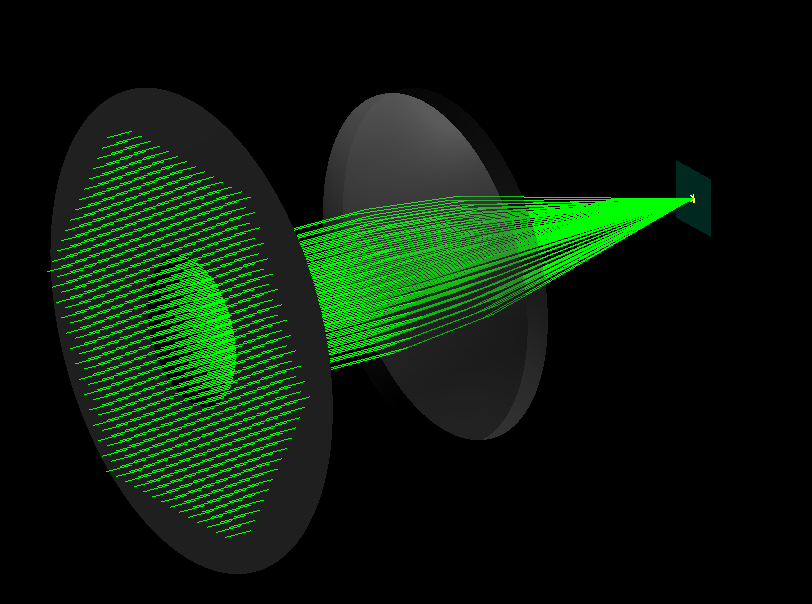
\includegraphics[width=0.75\textwidth]{images/ColimatedBeam.png}
\end{figure}


\begin{figure}[H]
    \caption{Photodiode Signal Filter}
    \centering
    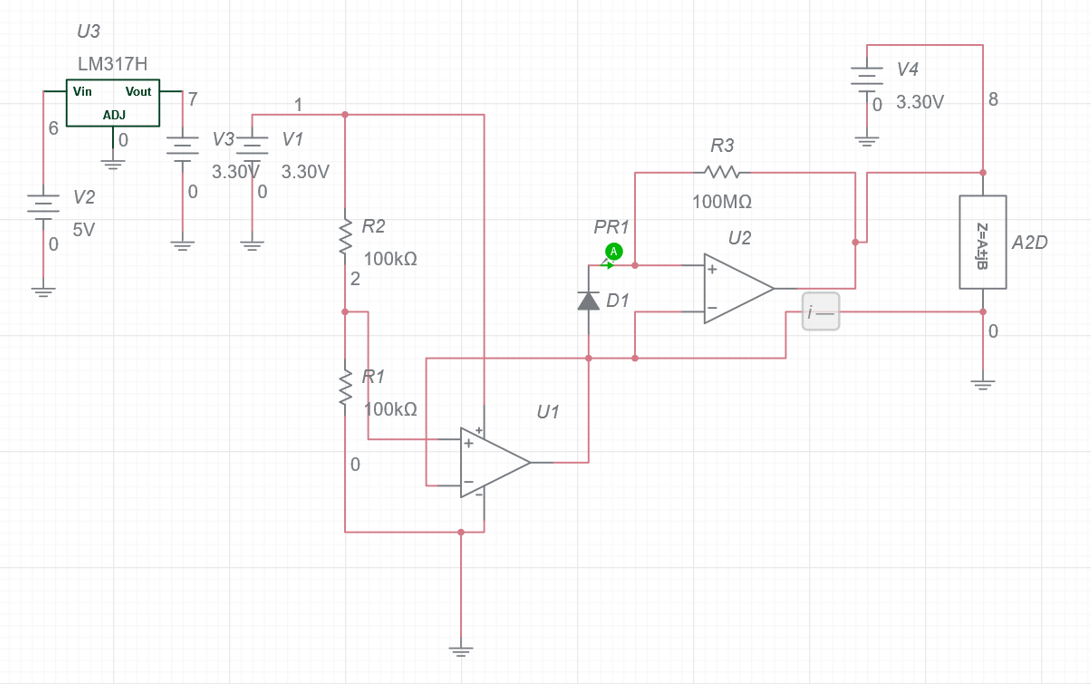
\includegraphics[width=0.75\textwidth]{images/ElectricalSignalFilteringSD1.png}
\end{figure}


The Photodiode works by converting a small portion of the incident light into electrical current across the face of the semiconductor. The diode will have a small current running through the circuit hooked up to an amplifier for boosting the signal to a detectable level. Then another op amp will cut out the electrical noise created by unwanted frequencies generated by the diode and electromagnetic interference.

              % Section 5.3
\subsection{Web Subsystem}
\label{sec:web_subsystem}
\begin{figure}[H]
    \caption{Web component block diagram}
    \centering
    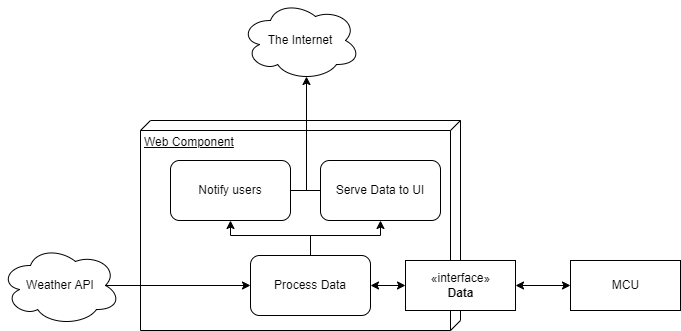
\includegraphics[width=\textwidth]{images/WebBlock.png}
\end{figure}                  % Section 5.4
\subsection{Subsystem Integration}
\label{sec:subsystem_integration}
The integration of all the subsystems is centered around the control subsystem. In the following sections, the team will discuss how these integrations will occur as the design process was centered around creating individual black boxes for each system to work against.

% TODO: Scott look this WHOLE SUBSECTION over and check if it's accurate.
\subsubsection{Sensing}
The sensing subsystem has three key components for the control subsystem to interact with: the linear rail and carriage the spectrometer is mounted to, the laser generating photons for the spectrometer to receive, and the spectrometer itself.

\paragraph{Linear Rail and Carriage} The spectrometer will be mounted to a carriage that may slide back and forth on the linear rail. The position of the carriage on the linear rail determines the wavelength of light sampled, and therefore the wavelength can be interpolated by the position of the stepper motor controlling the spectrometer carriage. It is a natural conclusion that the microcontroller will be able to direct the spectrometer to measure a specific wavelength by moving the stepper motor a certain number of predetermined steps. The microcontroller will sample the entire spectral range and compile this data to prepare to send to the web subsystem for processing.
% TODO: Scott please add how to calculate displacement on the linear rail from the wavelength we are trying to sample
\begin{equation}
    \label{equation:wavelen-dist}
\end{equation}

% TODO: SCOTT fix this paragraph, below the fiber optic we have no clue how you plan on making this work
\paragraph{Laser} The laser mounted to the Carriage will be commanded to power on by the microcontroller whenever the microcontroller wishes to obtain a sample from the spectrometer. The laser itself draws a minimal amount of current and is compatible with the voltages regulated and output by the microcontroller, and will simply be connected to one of the microcontroller's GPIO pins.

\paragraph{Spectrometer} The spectrometer itself will be stationary relative to the spectrometer's carriage. The spectrometer is a passive instrument that generates current depending on the flux density on the sensor. Due to the position of the spectrometer, this flux density is based on the strength of the specific wavelength emission. This current is connected to the sensing subsystem circuitry described in \ref{sec:sensing_subsystem}. This circuitry will proportionally convert the current to a voltage, and the output of the circuit will be connected to an analog-configured pin of the microcontroller, which will be taken as an input to the microcontroller's analog-to-digital converter. The ADC will convert the voltage to a value able to be measured in programming. The current (and by extension, voltage) level measured will be paired with the wavelength and transmitted by the MCU to the Amazon EC2 instance.

% TODO: Justin look this WHOLE SUBSECTION over and check if it's accurate.
\subsubsection{Power} The charge controller will deliver voltage of the battery to the microcontroller via

\subsubsection{Web}
The web and control subsystems interact via two way WebSocket protocol (\ref{websocket_protocol}), which will utilize TCP (\ref{tcp_standard}) as the transport layer protocol. Section \ref{sec:controller_subsystem} talks about the format of the raw texts in the packets. The web subsystem will be deployed to a fixed domain so the memory of the control system can use a fixed host for the Socket server. The socket server will always start by processing the address information of the incoming socket, and grabbing previous data from the database accordingly. The socket server will process the data, storing it in the database for reporting on later. If necessary, the socket server will send a request to the plant bed to do some function. This is laid out in \autoref{fig:web-control-sequence}.

\begin{figure}[H]
    \caption{Web--Plant Bed Socket Integration Sequence Diagram}
    \centering
    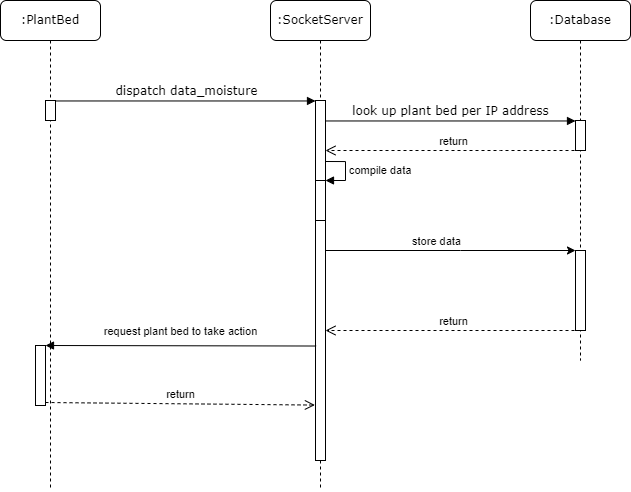
\includegraphics[width=.75\textwidth]{images/web-control-integration-sequence.png}
    \label{fig:web-control-sequence}
\end{figure}

          % section 5.5
\section{Testing}                               % Section 6 - add sections for individual test plans, and integration test
Incremental unit testing will be used during the development process
to ensure each subsystem fulfills design requirements as described in
\autoref{sec:??}. Controller subsystem testing will be performed in
\autoref{sec:controller_subsystem_testing}, power subsystem testing will be
performed in \autoref{sec:power_subsystem_testing}, sensing subsystem testing
will be performed in \autoref{sec:sensing_subsystem_testing}, and web subsystem
testing will be performed in \autoref{sec:web_subsystem_testing}. After
subsystems have fulfilled unit testing requirements, integration testing will
be performed with the criteria defined in \autoref{sec:integration_testing}.
\subsection{Controller Subsystem Testing}
\label{sec:controller_subsystem_testing}
The MCU subsystem will undergo a littany of testing. The electrical and
logical characteristics, as well as software behavior will be tested to ensure
a working product.

% Electrical characteristics (to see what it can handle and what it uses)
\paragraph{Electrical Characteristics}
Shutoff current testing \\
Hibernate current testing \\
Low power current testing \\
Active current testing \\
Shutoff voltage testing \\
Hibernate voltage testing \\
Low power voltage testing \\
Active voltage testing \\

% Logical characteristics (ability to set and use peripherals n stuff)
\paragraph{Logical Characteristics}
Upload code \\
I2C \\
LEDs \\
WDT \\
RTC \\
WiFi module \\
GPIO low/high \\
Interrupts/ISRs \\
ADC \\

% Software behavior (actual program)
\paragraph{Software Behavior}
Reset button \\
Connect to network \\
Connect to AWS \\
Receive over sockets \\
Send over sockets \\
Receive command from AWS \\
Send command to AWS \\
ISRs \\
                 % Section 6.1
\subsection{Power Subsystem Testing}
\label{sec:power_subsystem_testing}
\paragraph{}The Power subsystem is an important part in making sure that the whole system is fully operational. With various components such as the microcontroller, sensors, mechanical components and more, we need to make sure that each component is operating properly. In this section we will test ways to see if the components are compatible with each other and function properly. This is a confirmation that the whole system is operating but also a test to see which parts work best with each other and what works best under given situations. One thing that will be tested is the voltage regulators to see which of the selected voltage regulators is most efficient and regulate power the best see fit.	\par
\subsubsection{Solar Panel Testing}
\paragraph{}The solar panels in the system are very important because they essentially collect all the power for the system to operate. We will be testing and verifying that the open circuit voltage and the operating current are what they are supposed to be outputing in direct sunlight. \par
This is a quite simple test only needing the solar panels and a multimeter. To test the voltage coming out of the solar panel,we will be place it outside and we will grab the multimeter and set higher than the voltage that is said on the solar panel. Connecting the multimeter to the ends of the solar panel we can confirm the voltage that the solar panel should be outputing. The same steps are done to test the current that should be outputed from the solar panels.\par
\begin{figure}[H]
    \centering
    \caption{Solar Panel Testing}
    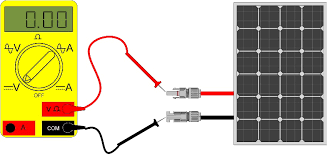
\includegraphics[width=\textwidth]{images/Solar_Panel_testing.png}
    \label{fig:Solar_Panel_testing}
\end{figure}
\subsubsection{Voltage Regulator}
\paragraph{}Providing power is an important part to operating a system, but providing the right amount of power is key to make sure all the components are operating properly. In this section we will test various designs from section 5 to see which of the designs for the given voltage regulators or from WEBENCH are best fit and most efficient. \par 
In this test, we will re-create the circuit designs that were in section 5, onto a breadboard using the right capacitors, resistors, and diodes. Then we will us an oscilloscope and a multimeter to measure the output voltages and currents for each design. This will help verify which circuit can regulate the voltage the best and most efficiently. \par
               % Section 6.2
\subsection{Sensing Subsystem Testing}
\label{sec:sensing_subsystem_testing}


There are three components in the Sensing subsystem that will require testing on arrival.
\begin{itemize}
    \item The Diffraction Grating
    \item The Optical Sensors
    \item The Linear Actuator
\end{itemize}


\paragraph{} The diffraction grating will be tested for efficiency and for line spacing. This will also determine if the blaze angle is correctly labeled.


\paragraph{} The photodiodes will be connected to circuitry and placed under beams to validate their responsivity curves and dark current.


\paragraph{} The linear actuator will be tested to ensure it responds properly to the specified voltage and current inputs and to ensure that it runs at the proper speed. Then the actuator will be tested to determine if the incremental steps are of the proper length.
             % Section 6.3
\subsection{Web Testing}
There are three components to test in the web system. The first is the API endpoints and backend functionality. The second is the integration of the user interface and the API. And lastly, the functionality of the socket server must be tested as well.
\subsubsection{API Testing} \label{sec:api-test}
There will be two key ways that the API testing will be conducted: unit tests and integration tests. In a web context these are slightly different than in a strict engineering context. Generally speaking, a unit test of a an API or backend service checks that business logic is working as expected. For example, in our project there will be some filter to grab the correct information from the database based on the plant bed. In a unit test, we might mock the database with dummy data and ensure that this is occurring properly.

On the other hand, the integration test of the API will be done in two ways which will also serve to self-document the API. Using a mock client, we can program requests for certain conditions such as certain failure or success. In this instance, the request is actually routed through all the middleware, connects to the database and performs the function. We can validate the result by looking at the database and ``asserting'' all these values are correct.

The self-documenting test will be done using Swagger and OpenAPI 3.0. Swagger is a tool for building UI elements that can build and run requests on the web server and the response elements can be validated against data types. See \autoref{fig:swagger} for a visual representation as to what this might look like.

\begin{figure}[H]
    \caption{Swagger UI example}
    \label{fig:swagger}
    \centering
    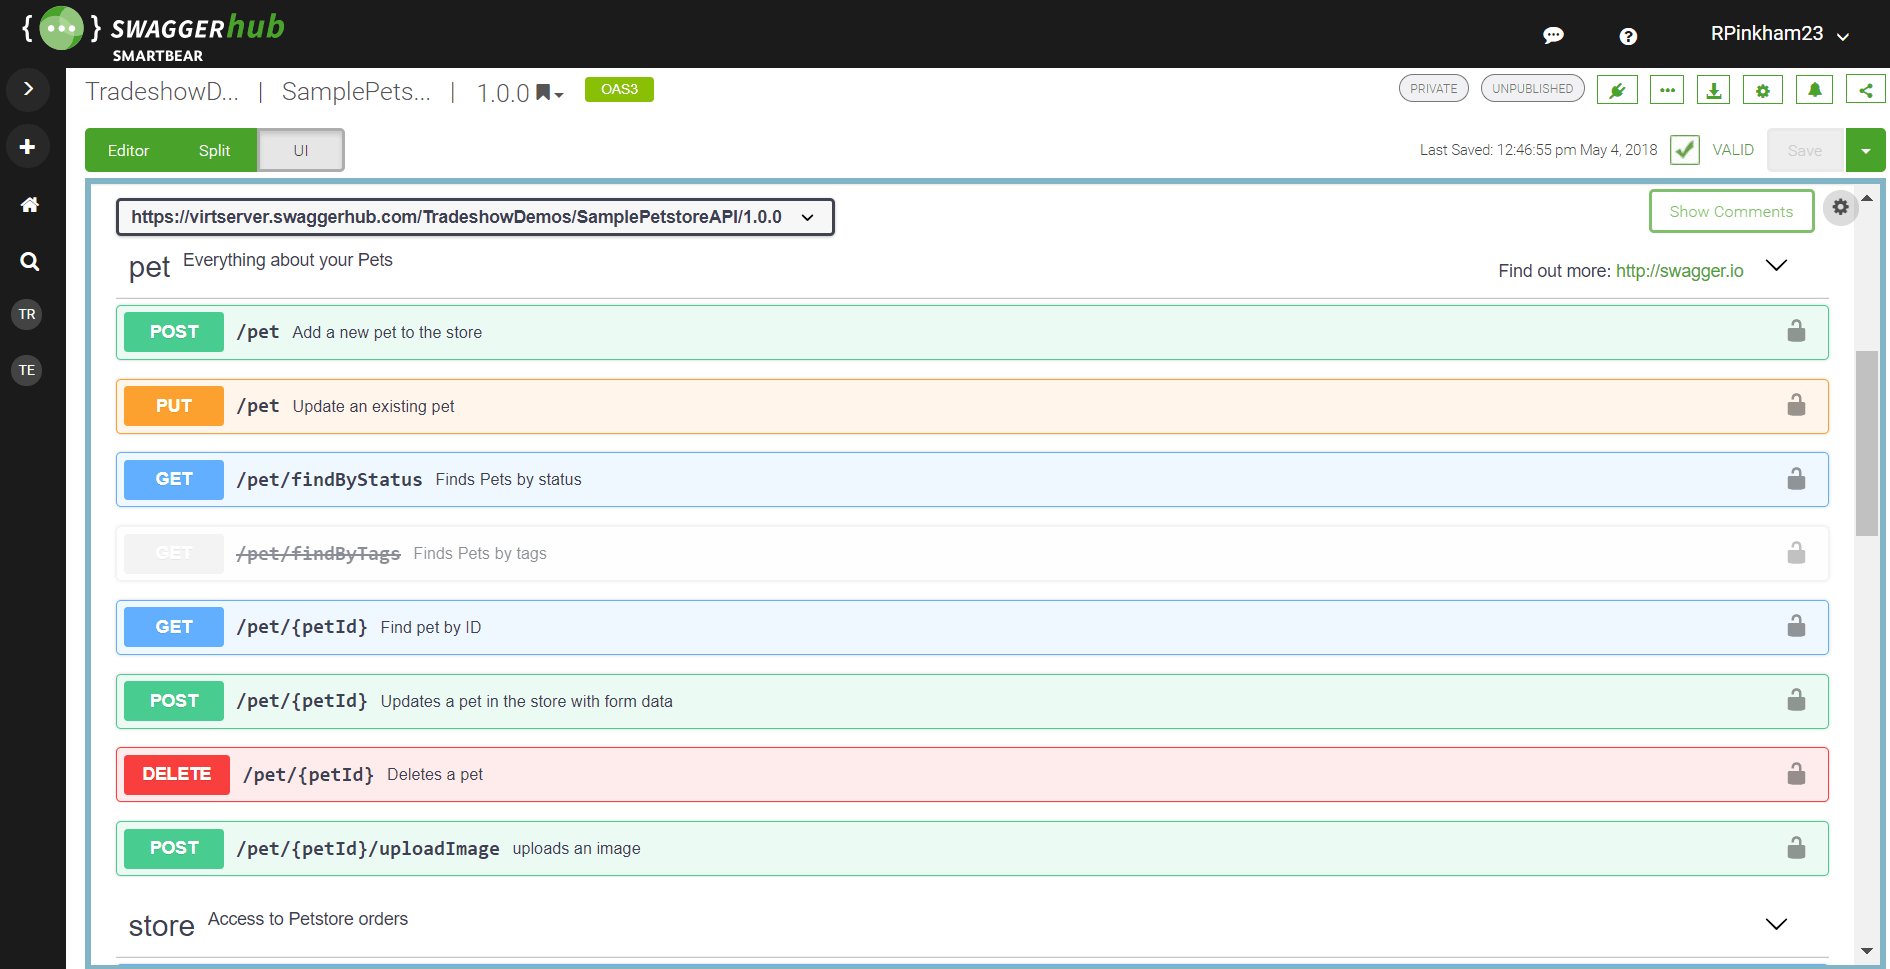
\includegraphics[width=\textwidth]{images/Swagger.png}
\end{figure}

\paragraph{Test Plan}
The unit tests and integration tests will be ran on each push of code changes to GitHub and through the use of GitHub actions, passing tests can be validated and added to the branch protection rules. Branch protection rules prevent broken code from becoming a part of the code base. These rules are integral to our test plan. See \autoref{fig:github-actions} to see how passing/failing tests would appear.

\begin{figure}[H]
    \caption{GitHub workflow}
    \label{fig:github-actions}
    \centering
    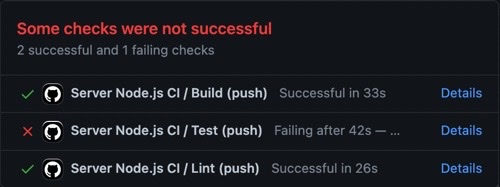
\includegraphics[width=\textwidth]{images/github.jpeg}
\end{figure}

The key to integrating this quality of life feature is designing good tests. The API in general has four functions: create, read, update, delete. The unit tests will be configured to ensure error handling and data composition are done properly. For example, when making a request about a particular plant bed, if the ID does not exist, we want to the error to be verbose but the request to fail. Similarly, we want to ensure that the logic for building data tables from the database occurs properly. The integration tests will have one well-formed request and one malformed request in order to test the error handling and full integration of correct data.

\subsubsection{User Interface Testing}
There are two key ways to be able test the user interface: using prototypes and integrating with the backend. Using React the expectation is that the user interface will be reactive. Thus, we use prototypes which are components built on hardcoded data that reacts to user input, thus we can test the viability of components. For example, we want to test that a graph component when hovered shows the data point in a floating box. We would build the UI with static data and ensure this result in the UI. Secondly, we need to test that the integration with the backend is working properly. This occurs by running an ``end-to-end'' test. Essentially, this is a final test. The plan is to give the testable product to consumers and let them have their way with the UI to discover bugs.

React comes packaged with a testing library that allows for quick unit testing of components in a similar way to the unit tests mentioned in the API section (\ref{sec:api-test}). Implementing this will automate the unit tests as opposed to manually building the entire program and checking manually each component. We will be using \href{https://testing-library.com/docs/react-testing-library}{this documentation} to build out the automatic test suite.

\subsubsection{Socket Testing}
Unit testing sockets will be done in a similar way to unit testing the API endpoints however the unit test will create a mock socket client and the two features will be tested separately: sending and receiving.

\paragraph{Sending Packets to Client}
To test that the client is receiving the packets properly in isolation, the mock client will open a connection to the server and the unit test will call the send packet function. The client will then expect certain values in a certain character set and this will all be validated by the assertion.
\paragraph{Receiving Packets from Client}
The mock client will send a packet to the socket server with static data that is formatted exactly as it would come from the MCU. From there, the unit test will assert that the received packet has all the required metadata, uses the correct character set and is formatted properly.
\subsection{Integration Testing}
\label{sec:integration_testing}
The microntroller is the key linkage between all the other subsystem's. Integration testing between these subsystems will be done in isolation before assembling the entire project. The integrations will be done and tested in the following order before a final full system test is completed.
\subsubsection{Web Integration}
Due to the use of Docker, the web integration test can be done at all points in development. There are two ways this can be done, downloading and running the image, or building the image from the source code. The processes for each are as follows:
\paragraph{Docker Image}
\begin{enumerate}
    \item Web developer uses docker to build the image
    \item Microcontroller developer downloads the built image from docker hub
    \item Use Docker Desktop to run image
    \item Test
\end{enumerate}
\paragraph{Build Docker Image from Source}
\begin{enumerate}
    \item Web developer pushes changes to Github
    \item Microcontroller developer pulls changes from Github
    \item Developer builds image from new source code
    \item Run the image and test
\end{enumerate}
\paragraph{Testing Areas}
There are two key areas that need to be test in this integration. First, that the microcontroller and web are communicating appropriately following the standards and design criteria. Second, that the microntroller is able to read and translate commands sent by the server and responds accordingly.

Through the use of UART on the microcontroller and verbose logging on the server application we can validate that the packets that are exchanged between the two systems are received and translated properly. Part of this test will be forcing packets to be sent, so the microcontroller will have commands in UART in order to force send packets to the web server so these can be verified. Similarly, the web component will need a way to force send packets to the microcontroller. These packets can be verified by looking at the metadata associated, the charset, length, and payload.

Once the packets have been verified we need to test that the microcontroller is responding to the packets it is being sent. This can be done in two ways. First, using UART we can print a response to the packet to show that the logic is working. The second part of this testing is ensuring digital logic on the pins to the control mechanisms are also working appropriately.

\subsubsection{Sensor Integration}
Sensor-controller integration shall be performed in the following manner. The sensing and controlling subsystems shall be connected according to the system schematics. This involves connecting the sensing subsystem power rail to V\textsubscript{CC}, as well as the sensing subsystem's V\textsubscript{out} to the MCU's analog-to-digital converter. The MCU shall be connected via backchannel UART to a compatible computer with a serial terminal for monitoring. The sensing subsystem shall be powered nominally and take samples on a timer providing regularly-timed samples for testing. Any raw values obtained shall be printed to the computer's serial terminal. The sensing subsystem shall measure a standardized sample, and the values obtained shall be compared against the known and calculated values of a standardized sample. Any error shall be calculated, and adjustments shall be made.

\subsubsection{Power Integration}
Power-controller integration shall be performed in the following manner. The sensing and power subsystems shall be connected according to the system schematics. This involves connecting the controller subsystem power rail to V\textsubscript{CC}, the MCU's SDA and SCL buses to the power subsystem's charge controller IC, and any analog lines in to the MCU's analog-to-digital converter to the power sensing and monitoring circuitry. The MCU shall be connected via backchannel UART to a compatible computer with a serial terminal. The power subsystem shall be providing power nominally, and testing shall be performed in the following conditions:
\begin{itemize}
    \item Battery 100\% charged, solar panels connected
    \item Battery 20\% charged, solar panels connected
    \item Battery 100\% charged, solar panels disconnected
    \item Battery 20\% charged, solar panels disconnected
\end{itemize}
Any voltage and current figures obtained shall be printed to the computer's serial terminal for monitoring. Any voltages and current figures measured shall fall within safe expected ranges. Any error shall be calculated, and adjustments shall be made.

\subsubsection{Full Integration}
After testing each of the individual integrations the final test will be seeing the whole system built and put together. The goal of the previous testing should be that there are issues with the code and the invidual parts. The full integration will consist of the following parts: power, control system tuning, usability.

\paragraph{Power}
In the previous testing sections the team has not yet covered a ``stress'' test of the power system. After integrating all the parts of the project, the team will do a 1 week trial run of the power system under an elevated load. This elevated load is more frequent scanning, longer duration of scanning, more transmissions to and from the web interface. This is in the hopes of tuning the power system and proving the viability of our power system. We can differentiate this stress test from lab tests due to the ``real world load'' that is being applied that could not have been tested until the completion of all the sections.

\paragraph{Control System Tuning}
The control system will need tuning with the sensor data. Models are only so good. The point of the control system tuning will be to measure soil water content against the sensor's interpretation of the soil moisture content as well as the checking the activation levels of the microcontroller. 

\paragraph{Usability}
The team will give friends and/or family the ability to demo the garden bed in person and from the website. They will have the following rubric to grade the project in order to help fix some of the usability shortcomings:

\begin{table}[H]
    \centering
    \caption{Usability Matrix}
    \begin{tabular}{|c|c|c|c|}
        \hline
        \textbf{Area} & \textbf{Metric} & \textbf{Grade} & \textbf{Notes} \\
        \hline
        \multirow{3}{*}{Web} & Navigable? & &\\
                        & Intuitive? & &\\
                        & Appealing? & &\\
        \hline
        \multirow{3}{*}{In-Person} & Durability? & & \\
                                & Setup? & & \\
                                & Satisfaction? & & \\
        \hline
    \end{tabular}
    \label{table:usability-matrix}
\end{table}

The team felt that the user experience was an essential part of a full integration test. This is a lengthy process but something that will be invaluable for further market research as well as simple improvements to UI. The in-person metrics will help the team evaluate whether they met their design goals or not.

         % Section 6.5
\section{Administrative Content}                % Section 7
\subsection{Milestones}
Our team has decided to utilize the Agile approach for this project. We chose this methodology because it allows our team to focus on sections of the project and aligns well with the semester schedule. By making iterations for this project internally, we are able to track our progress and make status updates. Another benefit of this will be tracking any delays or problems. If we are behind on a section, we have already planned ahead and allowed ourselves room for some variance. We are also using smaller deliverables for the project which gives us more tracking because we have more internal deadlines. We will be using Jira to track our progress and add reports throughout the process. We will also be utilizing Discord as a form of communication with each other. This will be a place where we can discuss any issues or ask quick questions when we are not in person. Below, we have a high-level breakdown written for our project goals.
\subsubsection{Fall}
\begin{itemize}
    \item COMPLETED: Select components for each subsystem
    \begin{itemize}
        \item Document selection reasoning
        \item Order to ensure on-time delivery
    \end{itemize}
    \item Model physical bed
    \begin{itemize}
        \item This item was not completed and will be added to Spring
    \end{itemize}
    \item Build physical bed
    \begin{itemize}
        \item This item was not completed and will be added to Spring
    \end{itemize}
    \item PARTIALLY COMPLETED: Understand how subsystems will integrate:
    \begin{itemize}
        \item Communication protocols (REST, I2C, SPI, DSP, etc)
        \item Power requirements
    \end{itemize}
    \item UI for Web subsystem
    \begin{itemize}
        \item This item was not completed and will be added to Spring.
    \end{itemize}
\end{itemize}
\subsubsection{Spring}
\begin{itemize}
    \item Model physical bed
    \item Build physical bed
    \item UI for Web subsystems
    \item Test subsystems in isolation
    \item Start integrating subsystems
    \item Control scheme for moving solar panels with sun and to provide shade
    \item Web API complete
    \item MCU coding complete
    \item Stretch goals
\end{itemize}

\subsection{Progress}

\subsubsection{Senior Design I}
\begin{figure}[H]
    \caption{Cumulative Flow Diagram from Jira}
    \centering
    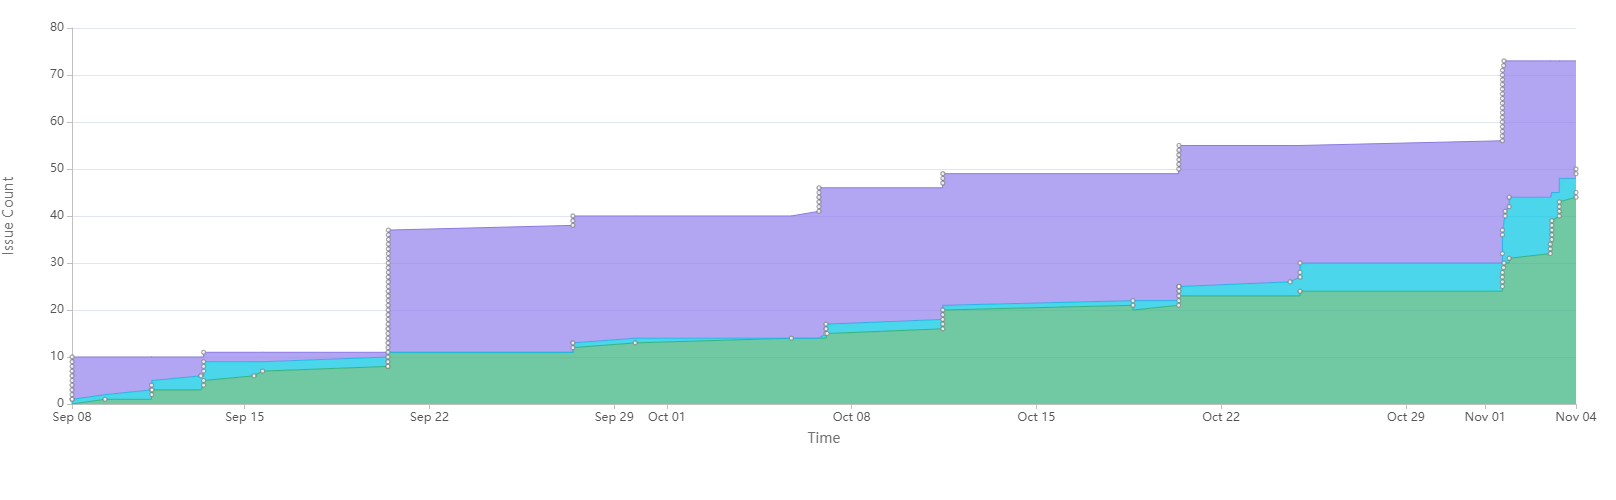
\includegraphics[width=\textwidth]{images/Cumulative flow diagram.png}
    \label{fig:cumulativeflow}
\end{figure}
In Figure \ref{fig:cumulativeflow}: purple designates tasks that are marked unfinished in the the backlog and current sprint, blue represents in progress tasks, and green represents finished tasks.

Throughout Senior Design I we have been gathering research and have started laying out the design of our garden bed and have completed the majority of our part selection. The Figure in \ref{fig:cumulativeflow} may be a little misleading at this point because we have not refined our backlog to fully encapsulate meaningful tasks instead breaking it down into larger subsystem requirement-esque tasks.
%Needs updating for SD2
            % Section 7.1 - refine backlog and move here, create gantt chart
\subsection{Budget}
\begin{table}[H]
    \centering
    \begin{tabularx}{.8\textwidth}
        {
            | >{\raggedright\arraybackslash}X
            | >{\raggedright\arraybackslash}X
            | >{\raggedleft\arraybackslash}X
            |
        }
        \hline
        Subsystem & Estimated Cost & Comment \\
        \hline
        MCU & \$60 & The MCU, wiring harness \\         % Changed 2022-09-29 by Brendan
        \hline
        Power & \$200 & Solar panels, batteries, control system \\
        \hline
        Sensing & \$100 & Components for sensing, optical sensors \\
        \hline
        Web & \$30 & Web service pricing \\             % Changed 2022-09-29 by Brendan
        \hline
        Non-Subsystem & \$100 & The plant bed, soil, water, fittings, etc \\
        \hline
        Total & \multicolumn{2}{|c|}{\$490}\\           % Changed 2022-09-29 by Brendan
        \hline
    \end{tabularx}
    \caption{Breakdown of budget by subsystem}
\end{table}               % Section 7.2 - update finances what was budgeted versus what was spent
\end{document}